% Copyright 2004 by Till Tantau <tantau@users.sourceforge.net>.
%
% In principle, this file can be redistributed and/or modified under
% the terms of the GNU Public License, version 2.
%
% However, this file is supposed to be a template to be modified
% for your own needs. For this reason, if you use this file as a
% template and not specifically distribute it as part of a another
% package/program, I grant the extra permission to freely copy and
% modify this file as you see fit and even to delete this copyright
% notice. 

\documentclass[xcolor=dvipsnames]{beamer}
\usepackage{bibentry}
\setbeamertemplate{bibliography item}{\insertbiblabel}
\usepackage{cancel}
\usepackage{amsmath} 
\usepackage{mathtools}
\newcommand{\norm}[1]{\left\lVert #1 \right\rVert}
% Command for round parenthesis
\newcommand{\roundP}[1]{\left( #1 \right)}
% Command for poisson brackets
\newcommand{\poisson}[2]{\left\lbrace #1, #2 \right\rbrace}

\usepackage{varwidth}
\usepackage{lipsum}
\usepackage{color}
\usepackage{todonotes}
\definecolor{dgray}{gray}{0.30}
\definecolor{uyellow}{RGB}{253,241,0}

\usepackage[utf8]{inputenc}
\usepackage{graphicx}
\usepackage{epstopdf}
\usepackage[english]{babel}
\usepackage{hyperref}
\usepackage{datenumber}
\usepackage{todonotes}
\usepackage{mathtools}
\usepackage{amsmath}
\usepackage{amssymb}
\usepackage{amsthm}
\usepackage[caption=true]{subfig}

\newtheorem*{thm}{Theorem}
\newcommand{\fmunu}{F^{\mu\nu}}
\newcommand{\E}{\vec{E}}
\newcommand{\B}{\vec{B}}
\newcommand{\rot}{\nabla\times}
\newcommand{\dive}{\nabla\cdot}
\newcommand{\tmunu}{T^{\mu\nu}}
\newcommand{\levichi}{\epsilon_{\mu\nu\sigma\gamma}}
\newcommand{\dete}{\textrm{det}}
\newcommand{\lna}{\textrm{ln}}
\newcommand{\Tr}{\textrm{Tr}}
\newcommand{\seno}{\textrm{sin}}

\makeatletter
\newcommand{\pushright}[1]{\ifmeasuring@#1\else\omit\hfill$\displaystyle#1$\fi\ignorespaces}
\newcommand{\pushleft}[1]{\ifmeasuring@#1\else\omit$\displaystyle#1$\hfill\fi\ignorespaces}
\makeatother



% There are many different themes available for Beamer. A comprehensive list with examples is given here:
% http://deic.uab.es/~iblanes/beamer_gallery/index_by_theme.html
%\usetheme{AnnArbor}
%\usetheme{Antibes}
%\usetheme{Bergen}
%\usetheme{Berkeley}
%\usetheme{Berlin}
%\usetheme{Boadilla}
%\usetheme{boxes}
%\usetheme{CambridgeUS}
\usetheme{Copenhagen}
%\usetheme{Darmstadt}
%\usetheme{default}
%\usetheme{Frankfurt}
%\usetheme{Goettingen}
%\usetheme{Hannover}
%\usetheme{Ilmenau}
%\usetheme{JuanLesPins}
%\usetheme{Luebeck}
%\usetheme{Madrid}
%\usetheme{Malmoe}
%\usetheme{Marburg}
%\usetheme{Montpellier}
%\usetheme{PaloAlto}
%\usetheme{Pittsburgh}
%\usetheme{Rochester}
%\usetheme{Singapore}
%\usetheme{Szeged}
%\usetheme{Warsaw}
%\usecolortheme{seagull}
%\usetheme{Malmoe} 

\setbeamercolor{frametitle}{fg=Black,bg=Blue!60}
\setbeamercolor{section in head/foot}{bg=Blue, fg=Black}
\setbeamercolor{author in head/foot}{bg=blue, fg=Black} 
\setbeamercolor{date in head/foot}{fg=blue} 
\setbeamercolor{institute in head/foot}{fg=Black}
\usecolortheme[named=Black]{structure}
\setbeamerfont{footnote}{size=\footnotesize}

\setbeamertemplate{}[page number] % To replace the footer line in all slides with a simple slide count uncomment this line
 
\title{\textbf{The Expected Shape of the Milky Way's Dark Matter Halos }}

% A subtitle is optional and this may be deleted
%\subtitle{Optional Subtitle}

\author{Jesus Prada}
% - Give the names in the same order as the appear in the paper.
% - Use the \inst{?} command only if the authors have different affiliation.

\institute[{\color{Black} Universidad de los Andes}] % (optional, but mostly needed)
{
 \normalsize Advisors:\\
 PhD Jaime E. Forero-Romero \\ \small Universidad de los Andes, Departamento de Física\\
  \vspace{5mm}
 \normalsize PhD Volker Springel \\ \small  Heidelberg's Institute of Theoretical studies
}
% - Use the \inst command only if there are several affiliations.
% - Keep it simple, no one is interested in your street address.

\tiny
\date{ \footnotesize May, 2018}
% - Either use conference name or its abbreviation.
% - Not really informative to the audience, more for people (including yourself) who are reading the slides online
	

\subject{The Expected Shape of the Milky Way's Dark Matter Halo}
% This is only inserted into the PDF information catalog. Can be left out. 

% If you have a file called "university-logo-filename.xxx", where xxx  is a graphic format that can be processed by latex or pdflatex, resp., then you can add a logo as follows:
% \pgfdeclareimage[height=0.5cm]{university-logo}{university-logo-filename}
% \logo{\pgfuseimage{university-logo}}

% Delete this, if you do not want the table of contents to pop up at the beginning of each subsection:
%\AtBeginSubsection[] { \begin{frame}<beamer>{Outline} \tableofcontents[currentsection,currentsubsection] \end{frame}}

% Let's get started
\begin{document}

\begin{frame}
  \titlepage
  \normalsize
\end{frame}
%--------------------------------------------
\begin{frame}{Outline}
 \tiny
 \tableofcontents
 \normalsize
  % You might wish to add the option [pausesections]
\end{frame}
%-------------------------------------------------------------------------------------------
\section{Motivation}
\begin{frame}
\centering
\Huge
\textbf{Motivation}
\normalsize
\end{frame}

\subsection{Evidences of Dark Matter}
\begin{frame}
\centering
\LARGE
\textbf{Evidences of Dark Matter (DM)}
\normalsize
\end{frame}
%--------------------------------------------------------------------------------------------
\begin{frame}
\centering
\large
\textbf{Rotation Curves}

\begin{figure}
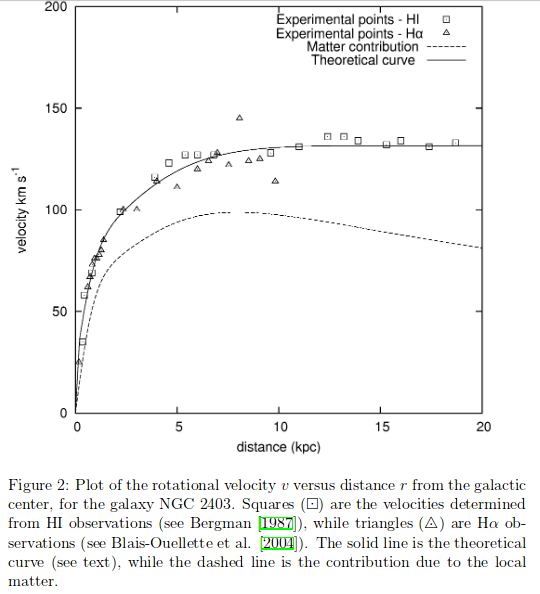
\includegraphics[width=0.6\linewidth]{./pics/RotationCurves.png}
\caption{\tiny Bertone et al. 2005}
\end{figure}

%\begin{itemize}
%\small
%\item Rotation curves
%\item Weak lensing
%\item CMB
%\item Large-scale structure of the universe
%\item Modified gravity
%\end{itemize}

\end{frame}
%--------------------------------------------------------------------------------------------
\begin{frame}
\centering
\large
\textbf{The Cosmic Background Radiation (Cold Dark Matter)}

\begin{figure}
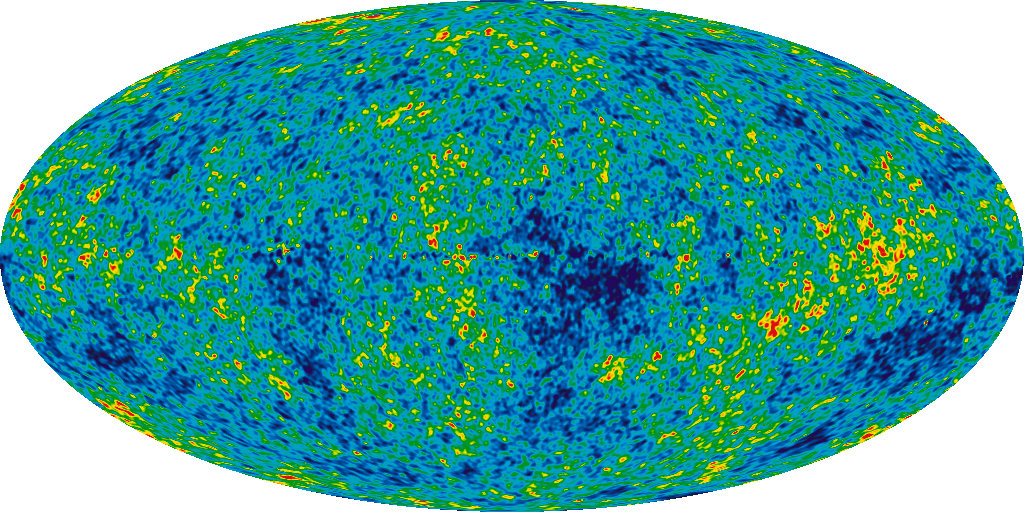
\includegraphics[width=1\linewidth]{./pics/CMB.png}
\caption{\tiny Taken from https://map.gsfc.nasa.gov/media/121238/index.html \textbf{(WMAP)}}
\end{figure}
\end{frame}

%--------------------------------------------------------------------------------------------
\begin{frame}
\centering
\large
\textbf{The Large-Scale Structure of the Universe}

\begin{figure}
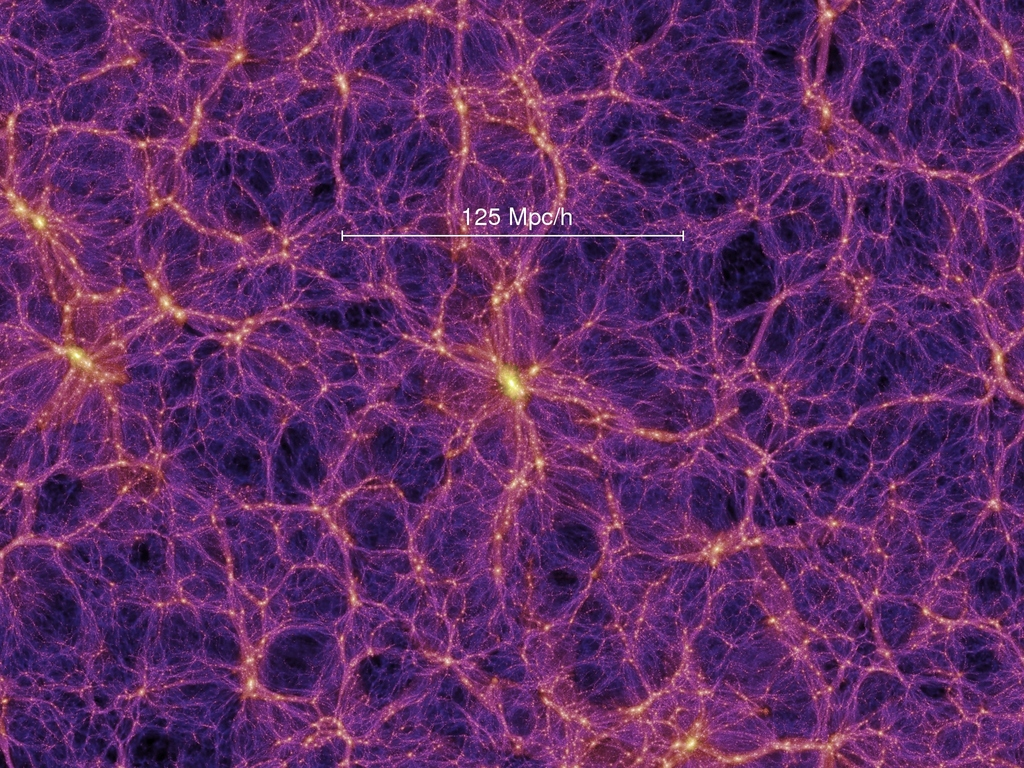
\includegraphics[width=0.6\linewidth]{./pics/LargeScale.jpg}
\caption{\tiny Taken from https://wwwmpa.mpa-garching.mpg.de/galform/virgo/millennium/ \textbf{(Millennium)}}
\end{figure}
\end{frame}

%--------------------------------------------------------------------------------------
\subsection{DM density in our Milky Way (MW)}
\begin{frame}
\centering
\LARGE
\textbf{DM density in our Milky Way (MW)}
\normalsize
\end{frame}

\begin{frame}
\large
\begin{itemize}
\small
\item \textbf{Why DM? --} We have not measured DM directly.\\~\\
\item \textbf{DM density field} is needed to couple theory and observations.\\~\\
\item DM evidence is not that far: MW\\~\\
\item \textbf{Why DM in our MW? -- }MW is the only object of which we have tridimensional view from the interior.
\end{itemize}
\normalsize
\end{frame}

%--------------------------------------------------------------------------------------------
\begin{frame}
\centering
\large
\textbf{MW is the only object of which we have tridimensional view from the interior}

\begin{figure}
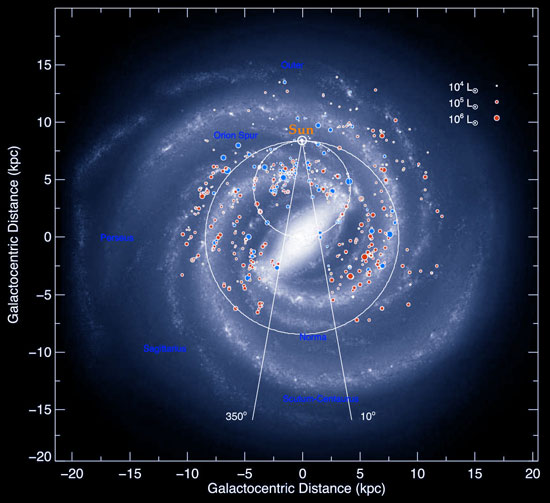
\includegraphics[width=0.55\linewidth]{./pics/MW.jpg}
\caption{\tiny Taken from https://imagine.gsfc.nasa.gov/science/objects/milkyway1.html \textbf{(Millennium)}}
\end{figure}
\end{frame}

%--------------------------------------------------------------------------------------
\subsection{Observational constraints on the MW's DM halo}


\begin{frame}
\centering
\LARGE
\textbf{Observational constraints on the MW's DM halo}
\normalsize
\end{frame}

%-----------------------------------------------------------------------------------------
\begin{frame}
\small

\begin{columns}[c]

\begin{column}{.5\textwidth}
\begin{figure}
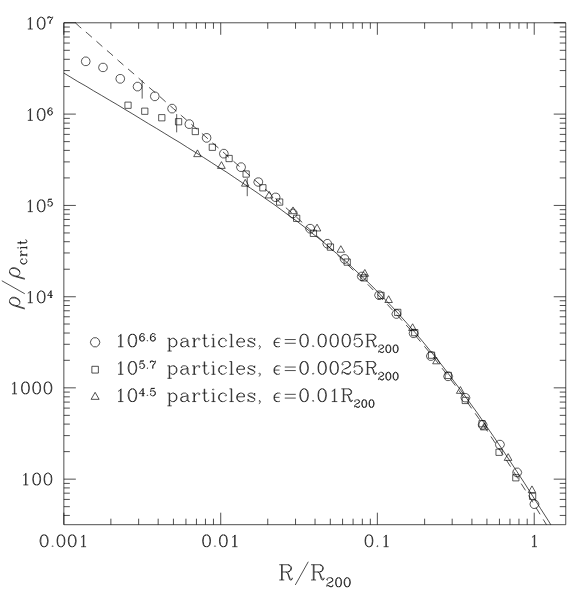
\includegraphics[width=0.8\linewidth]{./pics/radialProfile.png}
\caption{\tiny Gighna et al. 2000}
\end{figure}
\end{column}

\begin{column}{.6\textwidth}

The DM density field is often reduced to a radial profile:

\begin{equation}
\rho(\vec{r}) \rightarrow \rho(r) = \frac{\delta_c \rho_{crit}}{\frac{r}{r_c}\left( 1 + \frac{r}{r_c}\right)},
\end{equation}

which is universal in a hierarchical model of formation \cite{Navarro1997}.\\~\\

\end{column}

\end{columns}

\end{frame}

%---------------------------------------------------------------------------------------
\begin{frame}
Radial profiles omit angular dependence of density (\textbf{shape}).\\~\\

DM halos are NOT spherical but \textbf{triaxial} \cite{Allgood2006} (accretion)\\~\\

\begin{block}
{Why do we want to define a shape?}
Besides being a more complete characterization of density, it can keep memory of past events of formation.
\end{block}

\end{frame}
%---------------------------------------------------------------------------------------
\begin{frame}

\begin{columns}[c]

\begin{column}{.5\textwidth}
\begin{figure}
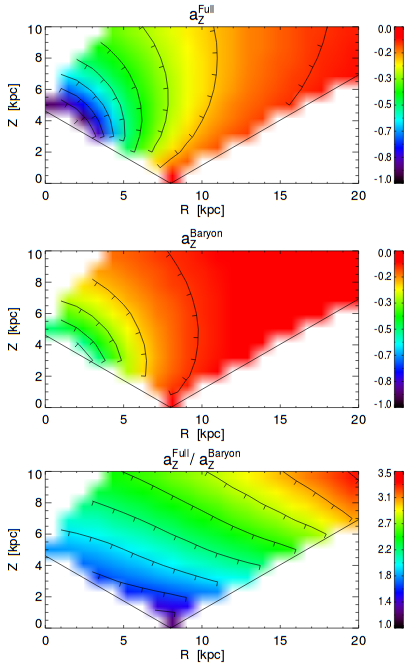
\includegraphics[width=1\linewidth]{./pics/loebmanAccelerationCurves.png}
\caption{\tiny Simulated $a_z$ comparison: Total Vs Baryon-contribution \\~\\\tiny Loebman et al. 2012}
\end{figure}
\end{column}

\begin{column}{.6\textwidth}
\centering
\small
\begin{itemize}

\item \cite[Loebman et al. 2012]{Loebman2012} deduced an oblate (\textbf{not spherical}) DM halo to account for discrepancies.

\end{itemize}

\end{column}

\end{columns}

\end{frame}
%---------------------------------------------------------------------------------------
\begin{frame}

\textbf{Using the Sagittarius stream} \cite[Law \& Majewski 2010]{LawMajewski2010}.

\begin{figure}[c]
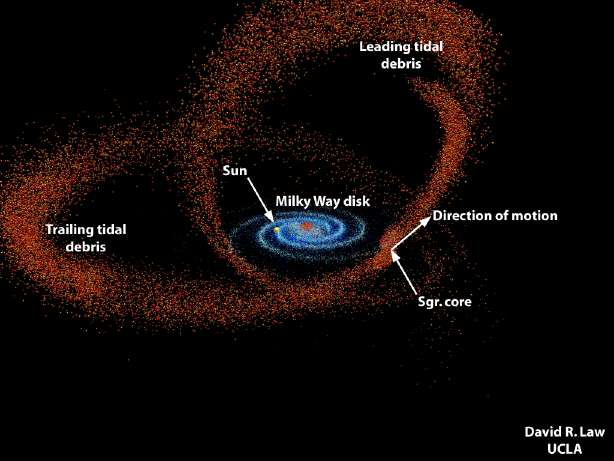
\includegraphics[width=0.6\linewidth]{./pics/Sagitarius.jpg}
\caption{\tiny Taken from https://phys.org/news/2017-07-astronomers-chemical-abundances-stars-nearby.html}
\end{figure}

\end{frame}

%---------------------------------------------------------------------------------------

\begin{frame}

\centering
\small
\begin{itemize}

\item \textbf{Variation of parameters}: Match simulations with observations.\\~\\

\item DM cannot be axisymmetric to account for the stream properties.\\~\\

\item DM halo is axisymmetric, nearly oblate.

\end{itemize}

\end{frame}

\begin{frame}
\centering
\textbf{Axis orientation??}
\begin{figure}[c]
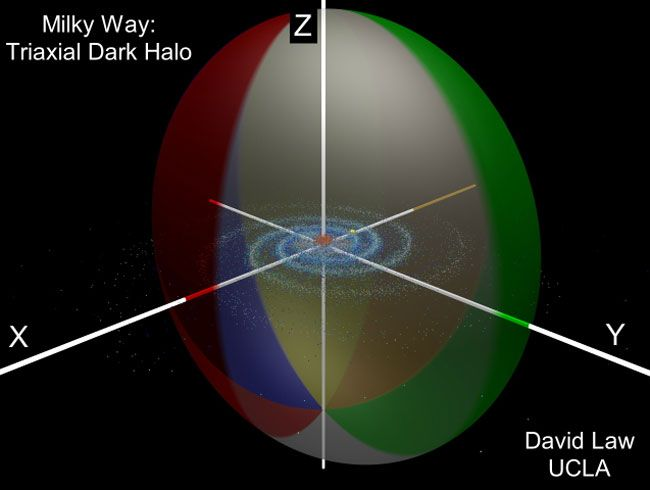
\includegraphics[width=0.6\linewidth]{./pics/MWDMHalo.jpg}
\caption{\tiny Taken from http://www.solstation.com/x-objects/darkhalo.htm}
\end{figure}

\end{frame}

%---------------------------------------------------------------------------------------
\subsection{The utility of Cosmological simulations}
\begin{frame}
\centering
\LARGE
\textbf{The utility of Cosmological simulations}
\normalsize
\end{frame}
%---------------------------------------------------------------------------------------

\begin{frame}

\begin{itemize}
\item Support tool for observation and theory.\\~\\

\item Evolution of DM and gas in a $\Lambda CDM$ cosmology\\~\\

\item Feedback processes: Supernovae explosions, Black hole radiation.\\~\\

\item Chemical enrichment\\~\\

\end{itemize}

\end{frame}

%---------------------------------------------------------------------------------------
%---------------------------------------------------------------------------------------
\begin{frame}

\begin{columns}[c]

\begin{column}{.5\textwidth}
\begin{figure}
\includegraphics[width=1\linewidth]{./pics/Auriga.png}
\caption{\tiny Auriga simulations. http://auriga.h-its.org}
\end{figure}
\end{column}

\begin{column}{.6\textwidth}
\centering
\footnotesize
\begin{itemize}


\item We focus on AURIGA \cite{auriga} simulations made with AREPO \cite{arepo}.\\~\\

\item \textbf{Degrees of realism}: Levels of Resolution. DM-only/Magneto HydroDynamics (MHD).\\~\\

\end{itemize}

\end{column}

\end{columns}

\end{frame}

%---------------------------------------------------------------------------------------
\subsection{Simulations and observations}
\begin{frame}
\centering
\LARGE
\textbf{Simulations and observations}
\normalsize
\end{frame}
%---------------------------------------------------------------------------------------

\begin{frame}
\centering
A study of the shape in terms of the radius: \cite[Vera-Ciro et al. 2011]{Vera-Ciro2011}.

\begin{figure}[c]
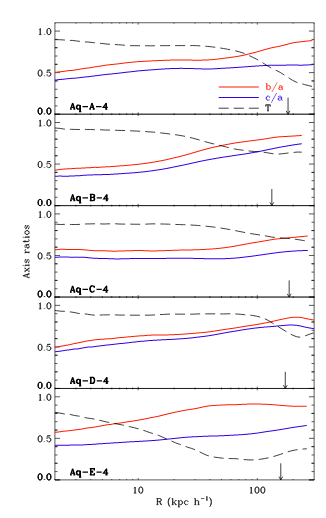
\includegraphics[width=1\linewidth]{./pics/shapeRadius.png}
\caption{ \tiny Halos evolve towards oblate shapes.  Vera-Ciro et al. 2011.}
\end{figure}

\end{frame}

%---------------------------------------------------------------------------------------

\begin{frame}
\centering
Correlation with historic shape.

\begin{figure}
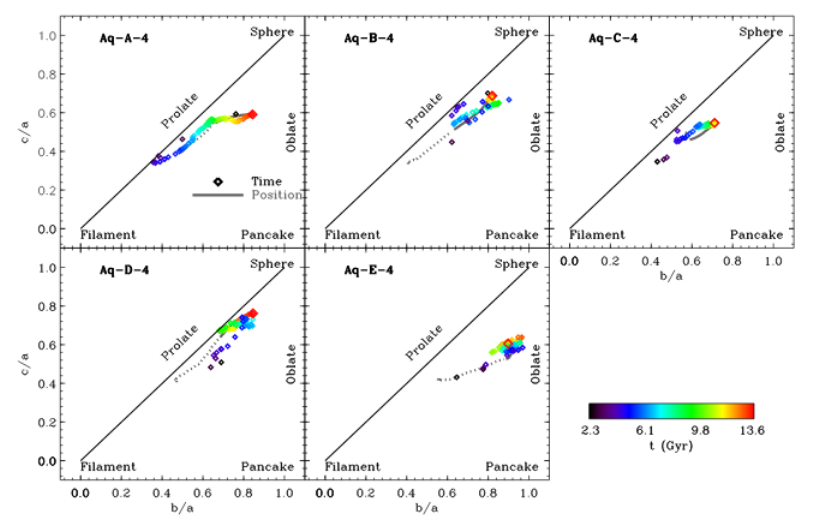
\includegraphics[width=1\linewidth]{./pics/shapeHistory.png}
\caption{\tiny Historical and radial correlation. Vera-Ciro et al. 2011}
\end{figure}

\end{frame}


%---------------------------------------------------------------------------------------
\begin{frame}

Improvement on observational constraints: \cite[Vera-Ciro and Helmi 2013]{Vera-Ciro2013}\\~\\

The DM halo assumptions:

\begin{itemize}
\item Axisymmetric at inner parts.\\~\\

\item Triaxial on the outer-skirts.\\~\\

\item Smooth transition.

\end{itemize}

\end{frame}

%---------------------------------------------------------------------------------------
%---------------------------------------------------------------------------------------
\section{Our study}
\begin{frame}
\centering
\Huge
\textbf{Our Study}
\normalsize
\end{frame}

\subsection{Objectives of this thesis}
\begin{frame}
\centering
\LARGE
\textbf{Objectives of this thesis}
\normalsize
\end{frame}

\begin{frame}

\begin{itemize}
\item Study the shape of the DM halo in terms of the radius on \textbf{AURIGA} simulations.\\~\\

\item Study the correlation of the radial and historical profiles.\\~\\

\item \textbf{\textit{Analyze the relation or the effect of baryons on the DM halo shape.}}

\end{itemize}

\end{frame}

%---------------------------------------------------------------------------------------
\subsection{The shape-calculation method}
\begin{frame}
\centering
\LARGE
\textbf{The shape-calculation method}
\normalsize
\end{frame}

\begin{frame}
\footnotesize
We follow Vera-Ciro et al. 2011 (\cite[Allgood et al. 2006]{Allgood2006}).\\~\\

Shapes are determined by the semiaxes $a,b,c$ of the halo ellipsoid.\\~\\

First we choose a radius $R$. We calculate the reduced inertia tensor for all particles within the defined sphere:

\begin{equation}
\Large
I_{ij} = \sum_k \frac{x_k^{(i)}x_k^{(j)}}{d^2_k}
\end{equation}

But this is not sufficient: \textbf{Spherical bias}.

\end{frame}


%---------------------------------------------------------------------------------------
\begin{frame}
\small

We recalculate by iteratively rescaling:\\~\\

Once obtained the first semiaxes, we perform the scale transform:

\begin{align}
(x,y,z) &\rightarrow (x,y/q,z/s) \\
q &=  b/a\\
s &= c/a,
\end{align}

This redefines the \textit{sphere} contour and the \textit{distance} in the inertia tensor.\\~\\

\textbf{Repeat until convergence}: changes in semiaxes are less than $10^{-6}$


\end{frame}

%---------------------------------------------------------------------------------------
\subsection{Convergence analysis}
\begin{frame}
\centering
\LARGE
\textbf{Corvergence analysis}
\normalsize
\end{frame}


\begin{frame}
\centering
Resolution does not visibly affect DM-only halo shapes.
\begin{figure}[!ht]
  \centering
  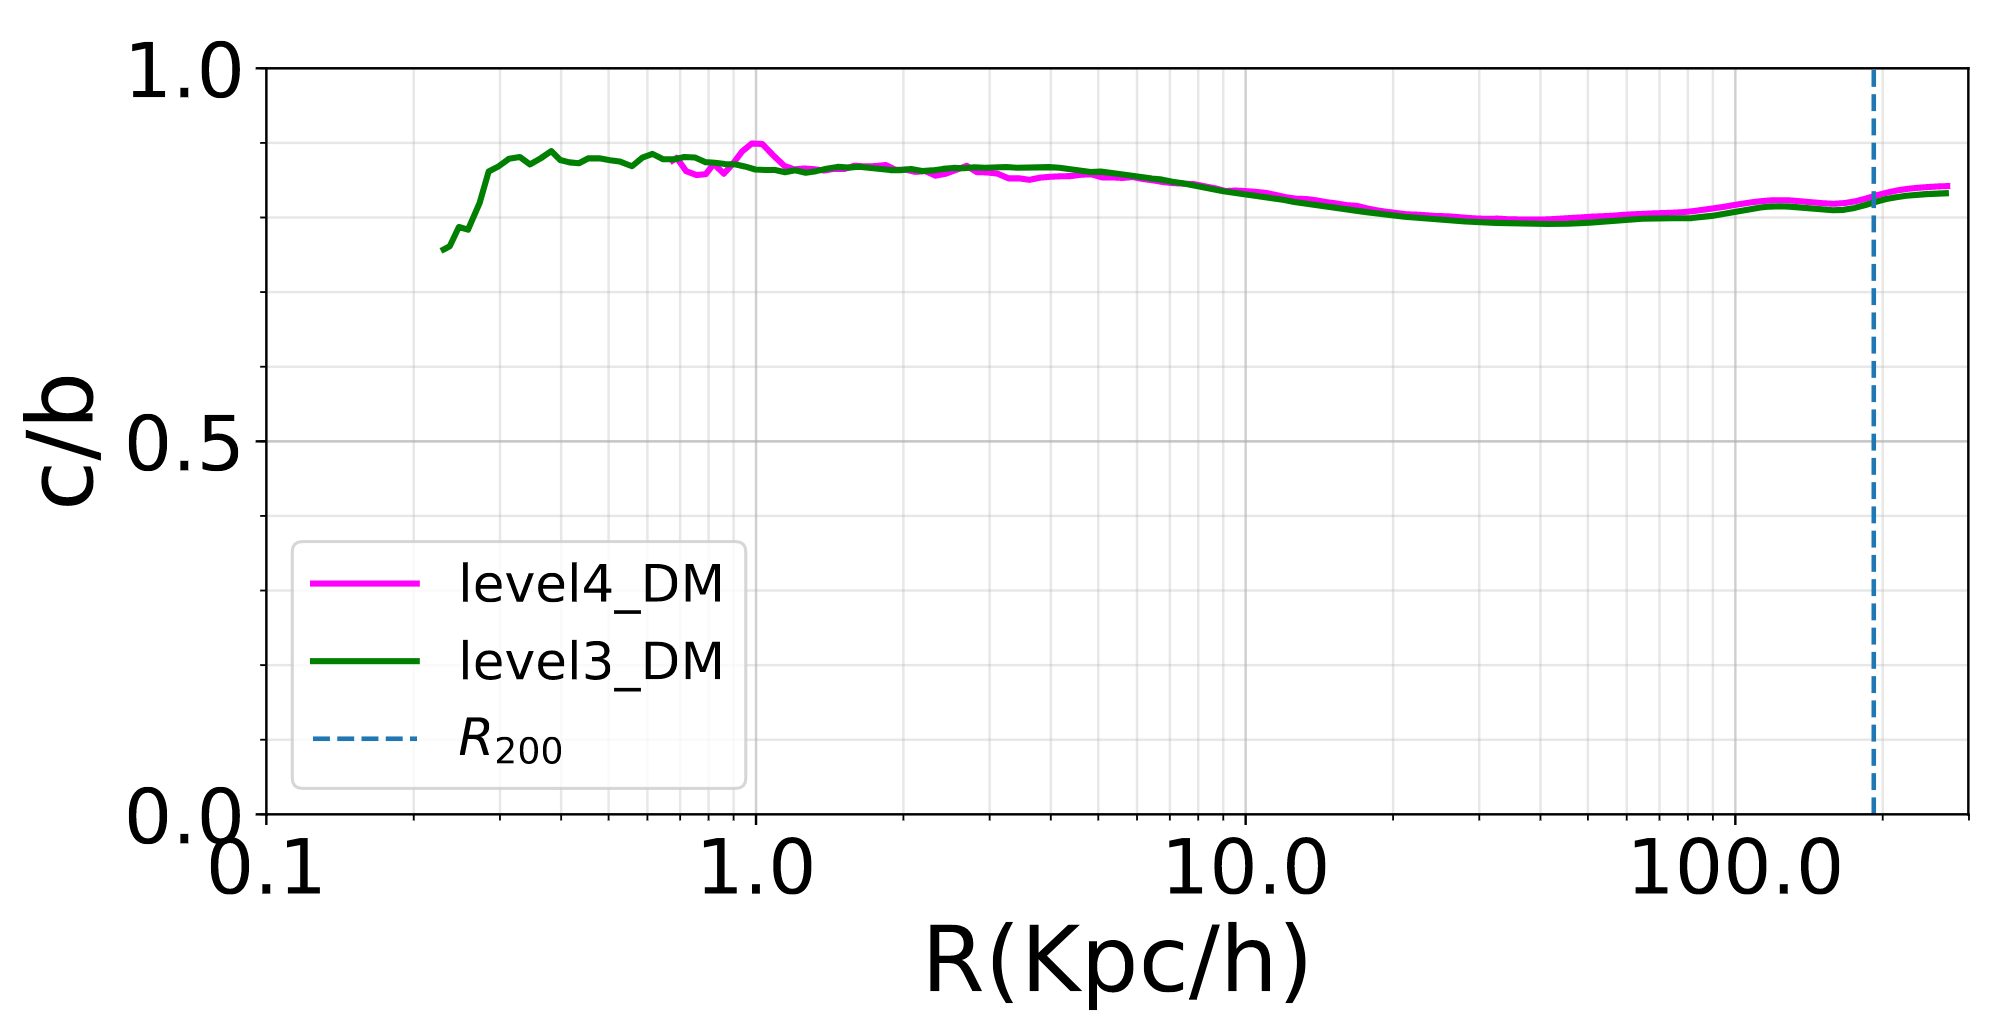
\includegraphics[width=1\columnwidth]{./pics/halo6_DM_3Vs4_good.png}
  \caption{Halo 6 DM \tiny Prada et al. 2018 (in process)}
  
\end{figure}
\end{frame}


\begin{frame}
\centering
MHD are affected by baryionic physics resolution (rather than a few-particle effect)
\begin{figure}[!ht]
  \centering  
  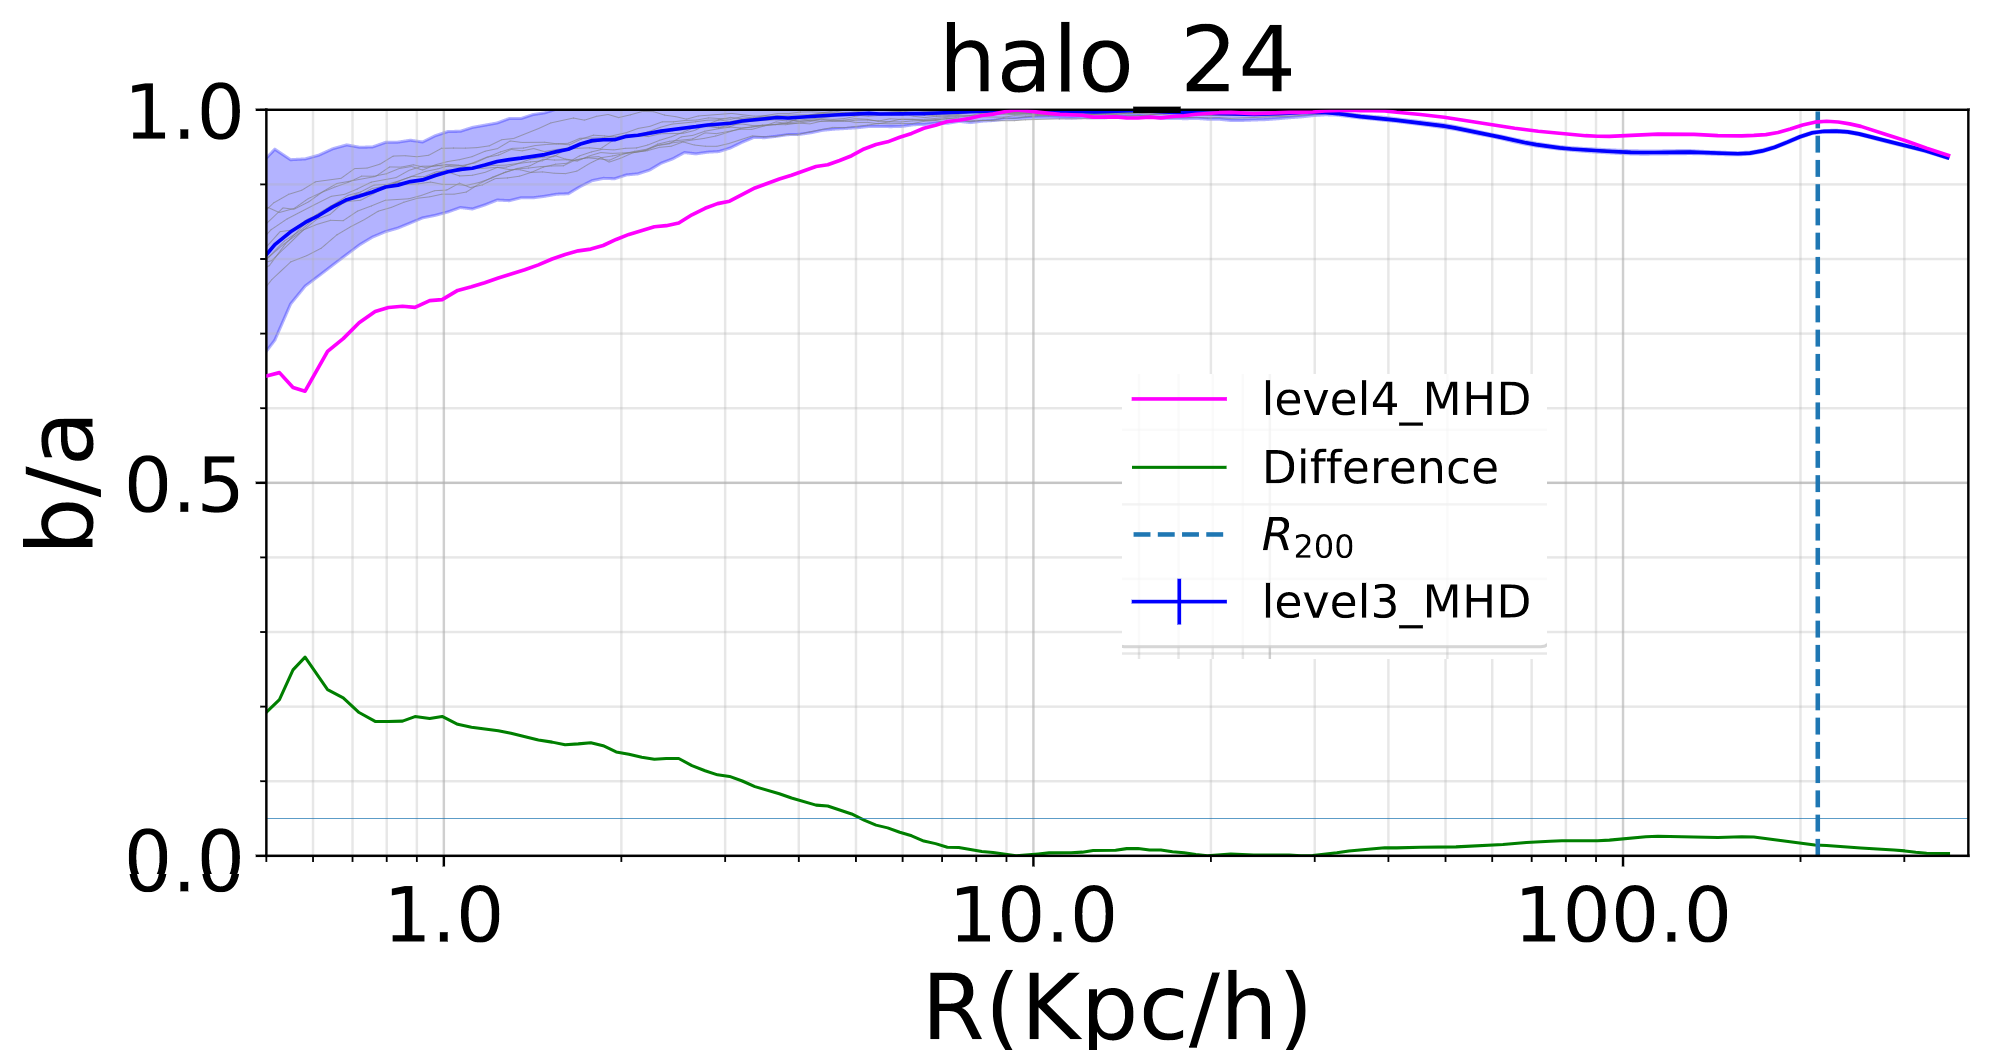
\includegraphics[width=1\columnwidth]{./pics/rand_conv_halo24_MHD.png}
  \caption{Halo 24 MHD \tiny Prada et al. 2018 (in process)}
\end{figure}
\end{frame}

%---------------------------------------------------------------------------------------

%---------------------------------------------------------------------------------------
\subsection{Radial dependence of shape}
\begin{frame}
\centering
\LARGE
\textbf{Radial dependence of shape}
\normalsize
\end{frame}

\begin{frame}[plain]

\begin{figure}[!ht]
  \centering
  \subfloat[\tiny halo 27 DM shape (inner)]{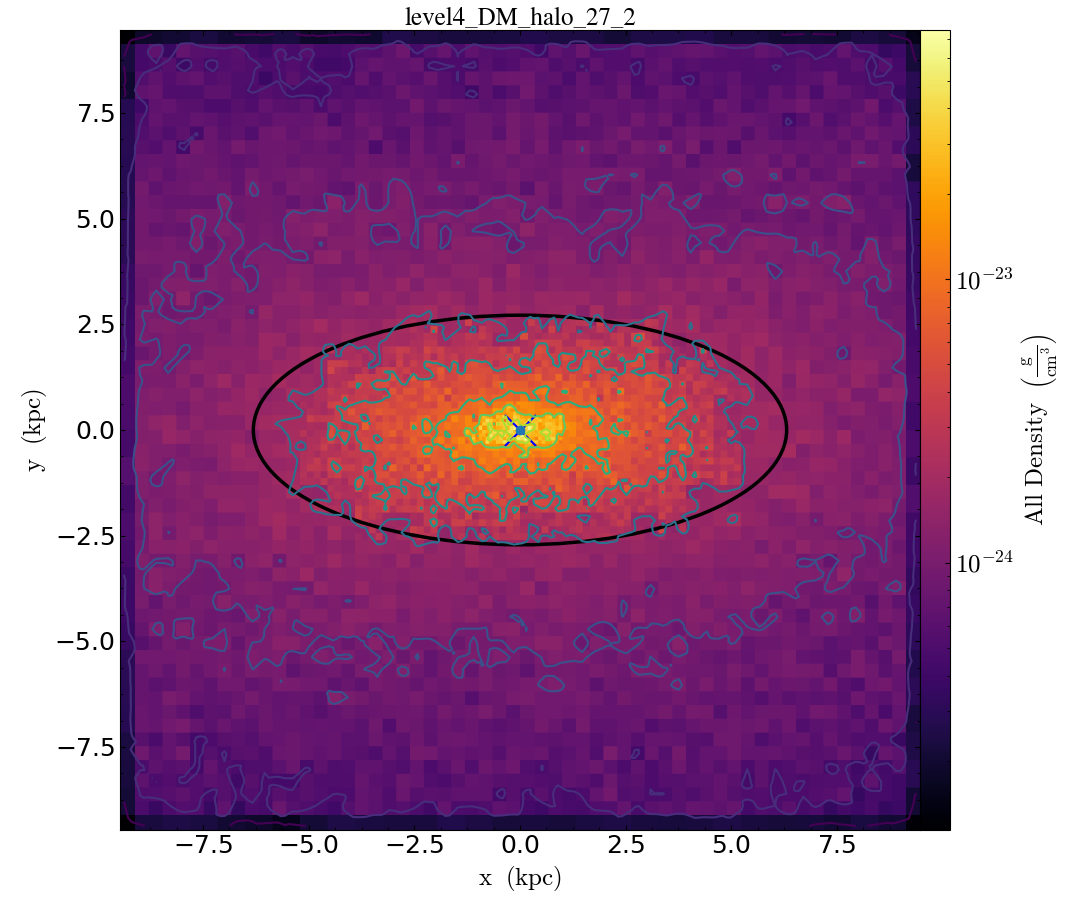
\includegraphics[width=0.38\columnwidth]{../Document/pics/MHD_Vs_DM/level4_DM_halo_27_inner.png}}
  \hfill %\HUGE DM
  \subfloat[\tiny halo 27 DM shape (outer)]{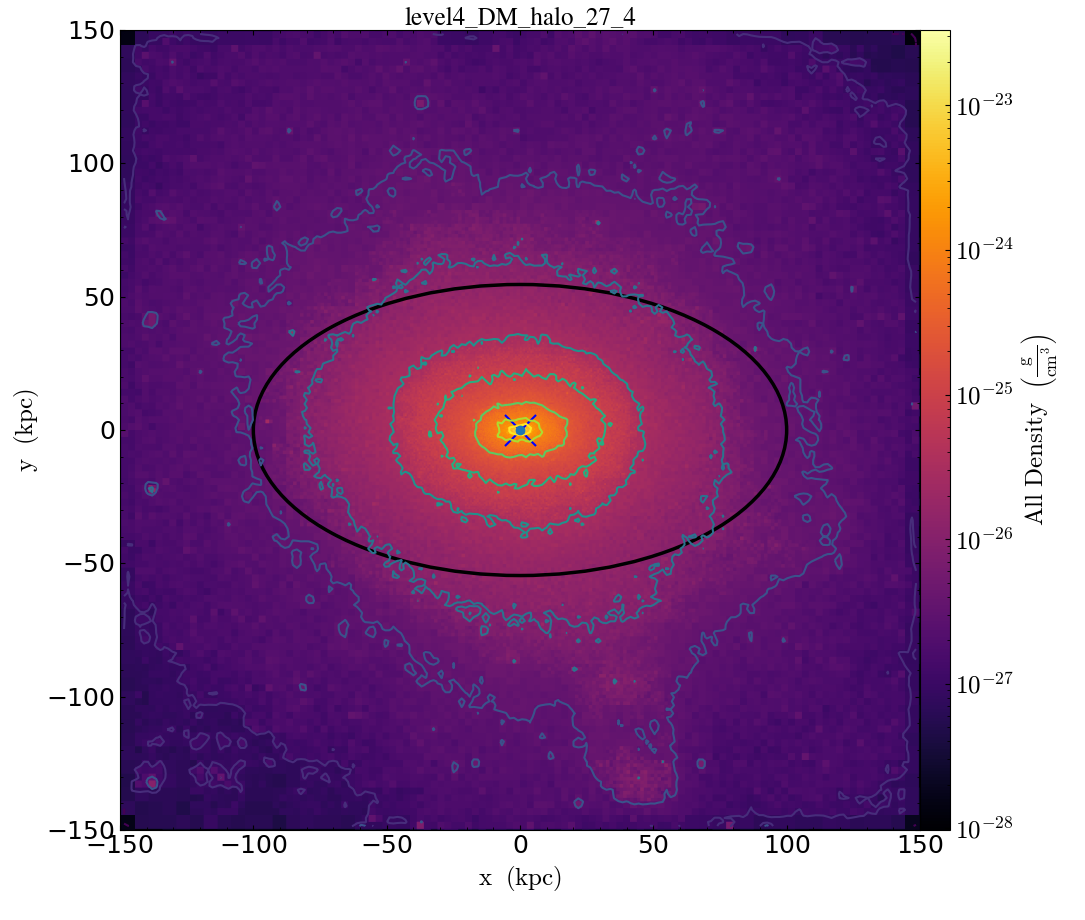
\includegraphics[width=0.38\columnwidth]{../Document/pics/MHD_Vs_DM/level4_DM_halo_27_outter.png}}
  \hfill
  \subfloat[\tiny halo 27 MHD shape (inner)]{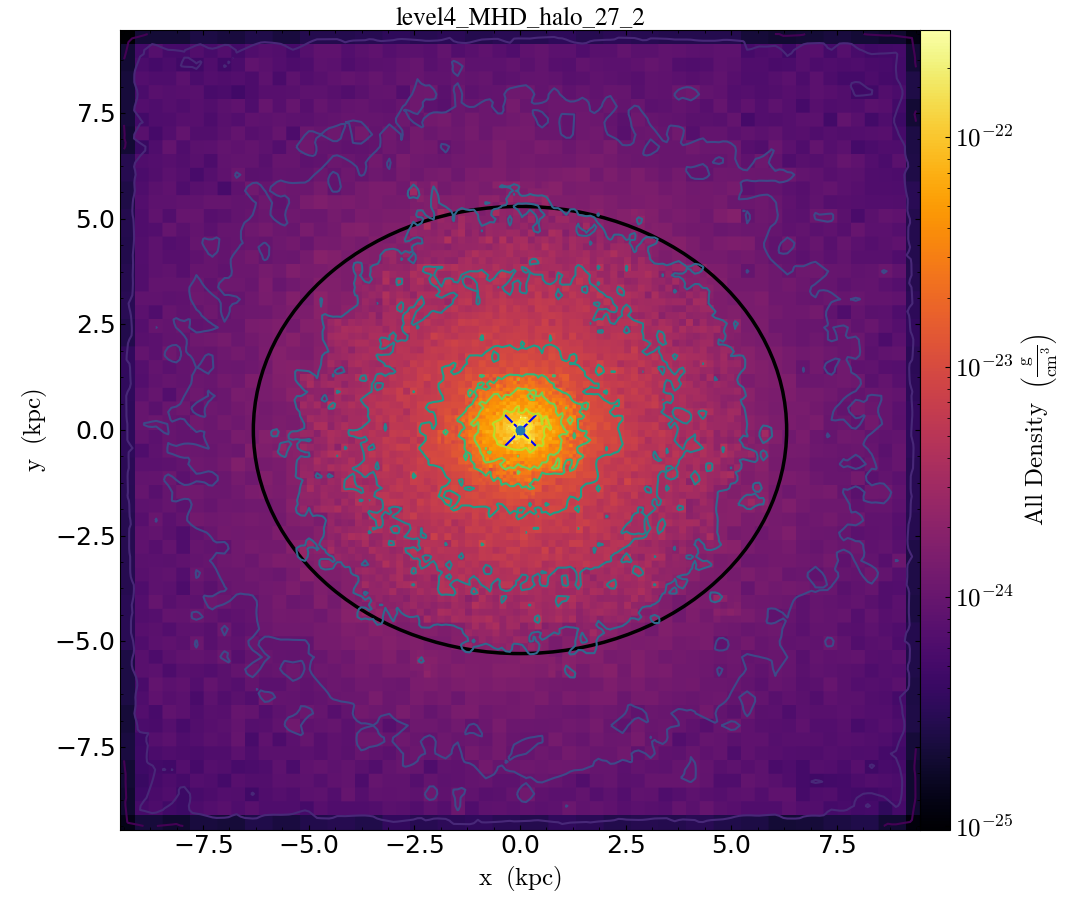
\includegraphics[width=0.38\columnwidth]{../Document/pics/MHD_Vs_DM/level4_MHD_halo_27_inner.png}}
  \hfill %\HUGE MHD
  \subfloat[\tiny halo 27 MHD shape (outer)]{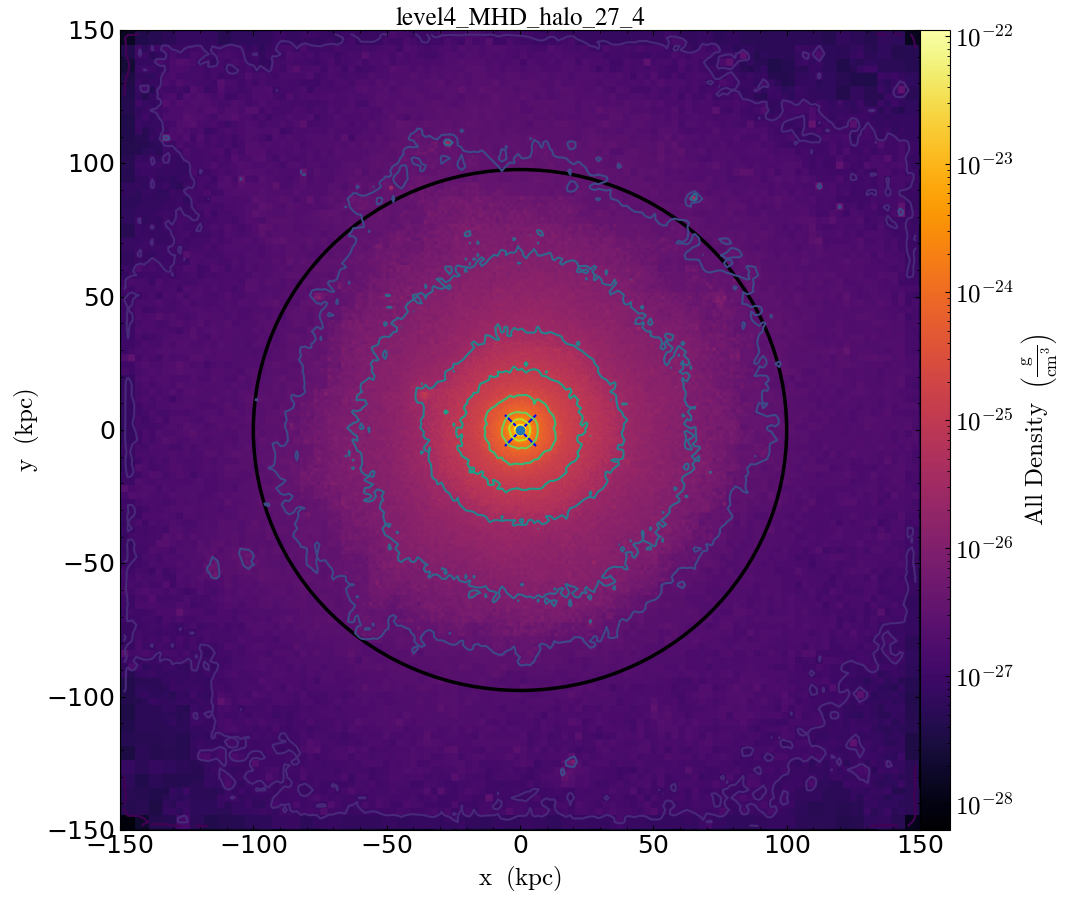
\includegraphics[width=0.38\columnwidth]{../Document/pics/MHD_Vs_DM/level4_MHD_halo_27_outter.png}}
 % \caption{DM density for inner (left) and outer (right) parts of the halo 27. We present both versions: DM (up) \& MHD (down). The horizontal and vertical axes are aligned to the major and medium semi-axes respectively. Here, it is evident that this halo is more spherical at bigger radii and more triaxial at the central parts. }
\normalsize
  \label{fig:slices}
\end{figure}
\centering
\tiny Prada et al. 2018 (in process)


\end{frame}

%---------------------------------------------------------------------------------------

\begin{frame}

\centering
DM Halos are more spherical at larger radii
\begin{figure}[!ht]
  \centering
  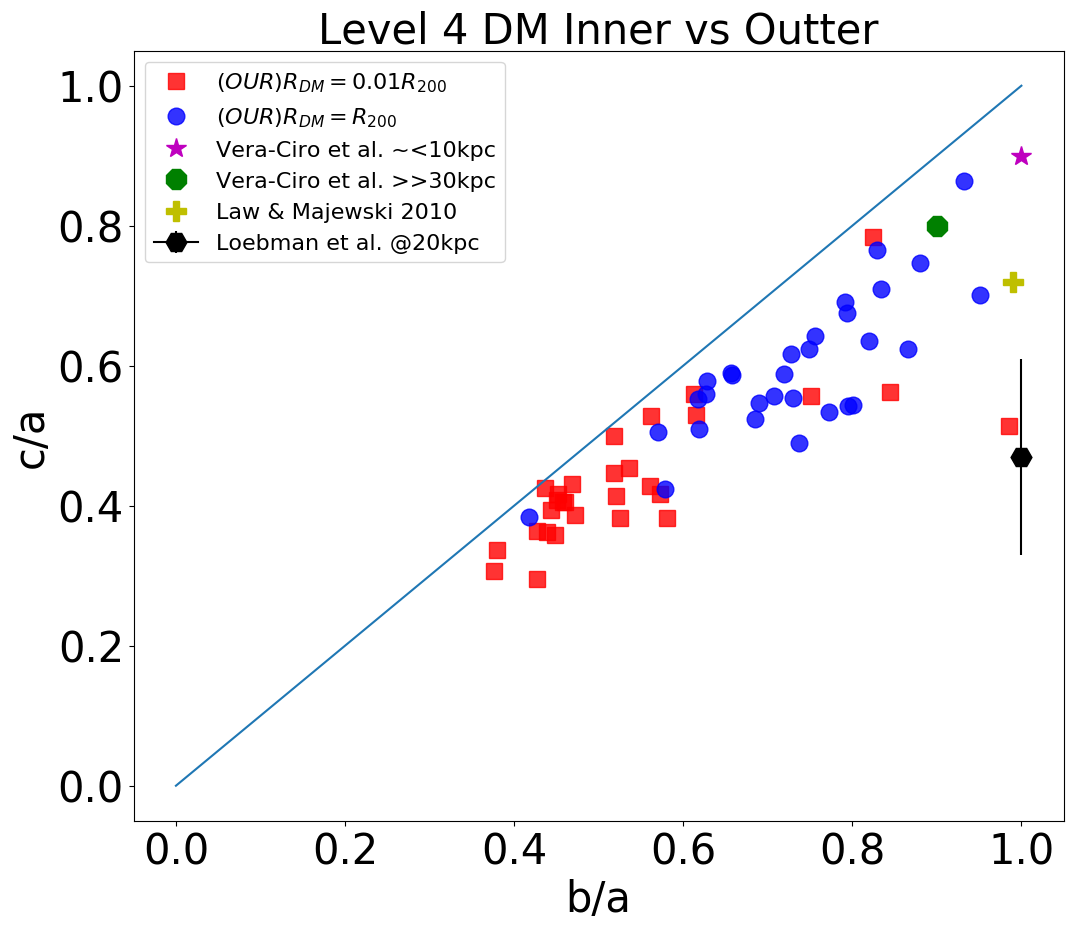
\includegraphics[width=0.6\columnwidth]{./pics/Triaxiality_DM_lvl4.png}
  \hfill
  \caption{\tiny Prada et al. 2018 (in process)}
\end{figure}
\normalsize

\end{frame}

\begin{frame}

\centering
MHD Halos are more spherical at larger radii
\begin{figure}[!ht]
  \centering
  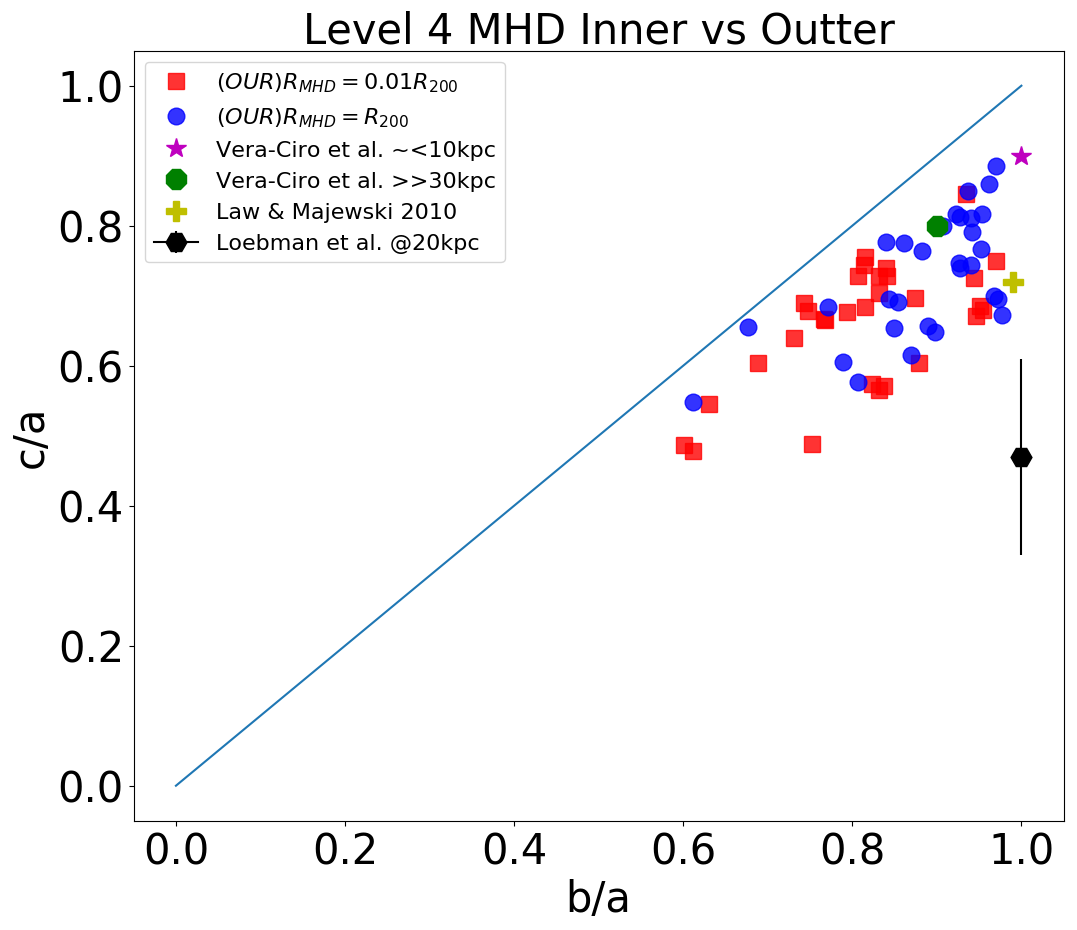
\includegraphics[width=0.6\columnwidth]{./pics/Triaxiality_MHD_lvl4.png}
  \caption{\tiny Prada et al. 2018 (in process)}
  \hfill

\end{figure}
\normalsize

\end{frame}

%---------------------------------------------------------------------------------------
\subsection{The effect of gas}
\begin{frame}
\centering
\LARGE
\textbf{The effect of gas}
\normalsize
\end{frame}

\begin{frame}[plain]

\begin{figure}[!ht]
  \centering
  \subfloat[\tiny halo 27 DM shape (inner)]{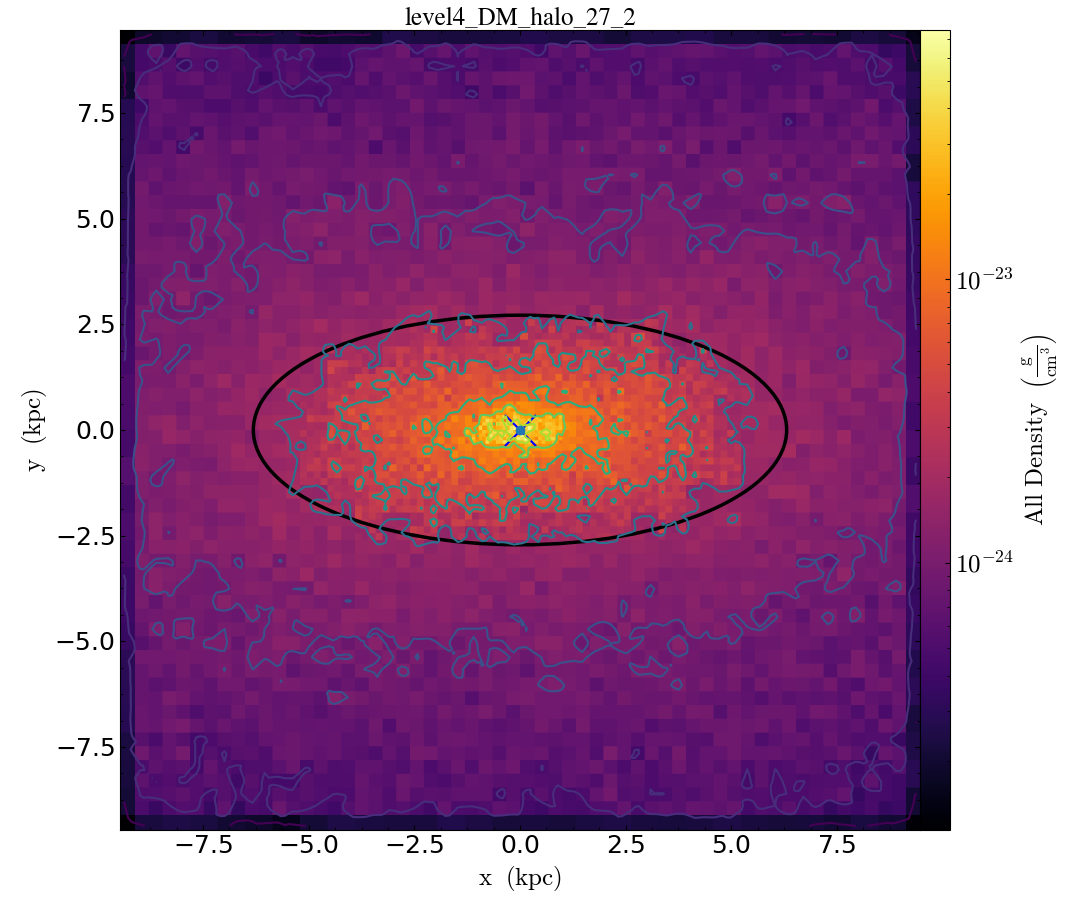
\includegraphics[width=0.38\columnwidth]{../Document/pics/MHD_Vs_DM/level4_DM_halo_27_inner.png}}
  \hfill
  \subfloat[\tiny halo 27 DM shape (outer)]{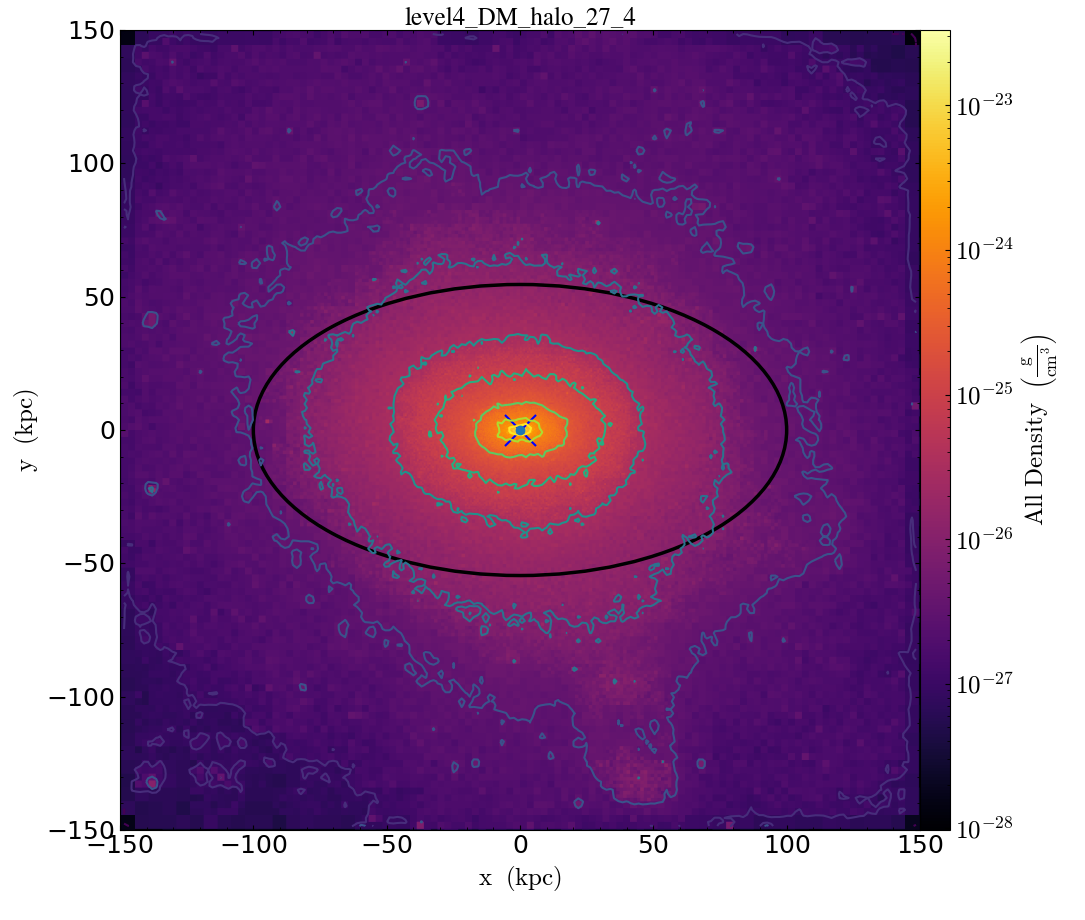
\includegraphics[width=0.38\columnwidth]{../Document/pics/MHD_Vs_DM/level4_DM_halo_27_outter.png}}
  \hfill
  \subfloat[\tiny halo 27 MHD shape (inner)]{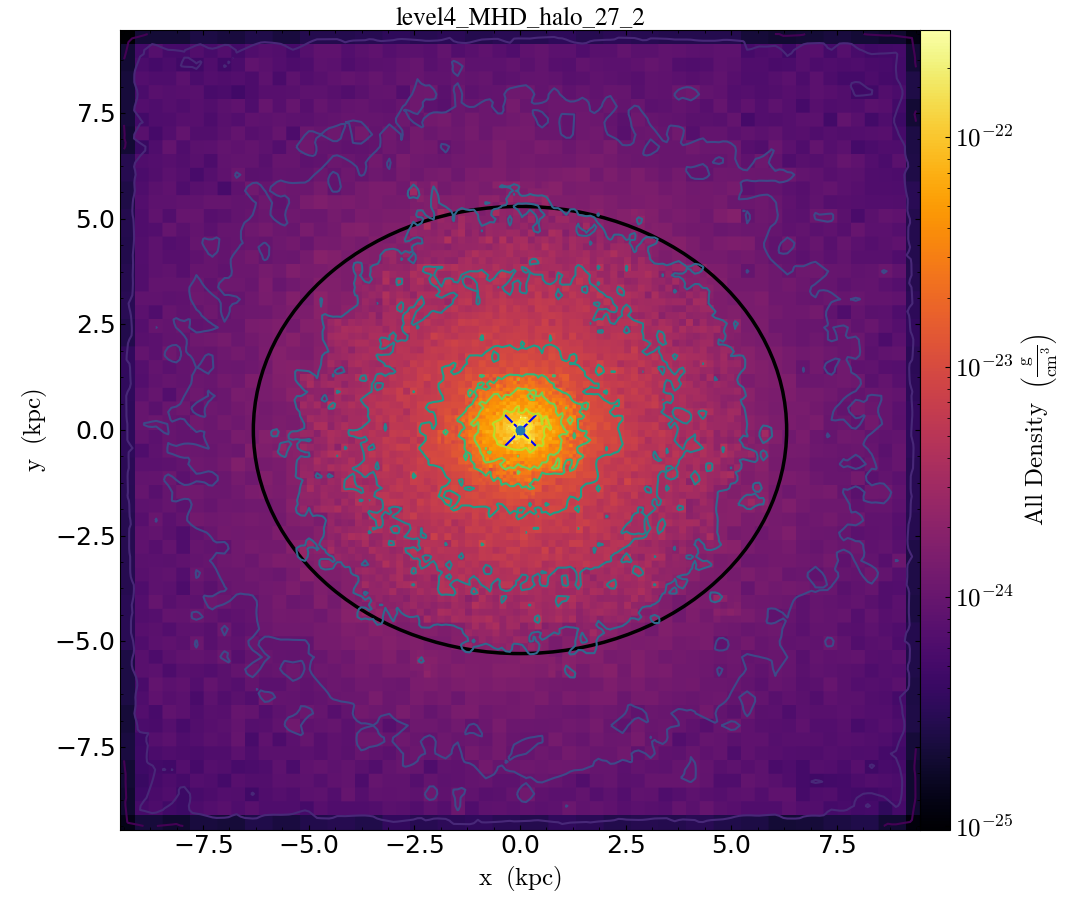
\includegraphics[width=0.38\columnwidth]{../Document/pics/MHD_Vs_DM/level4_MHD_halo_27_inner.png}}
  \hfill
  \subfloat[\tiny halo 27 MHD shape (outer)]{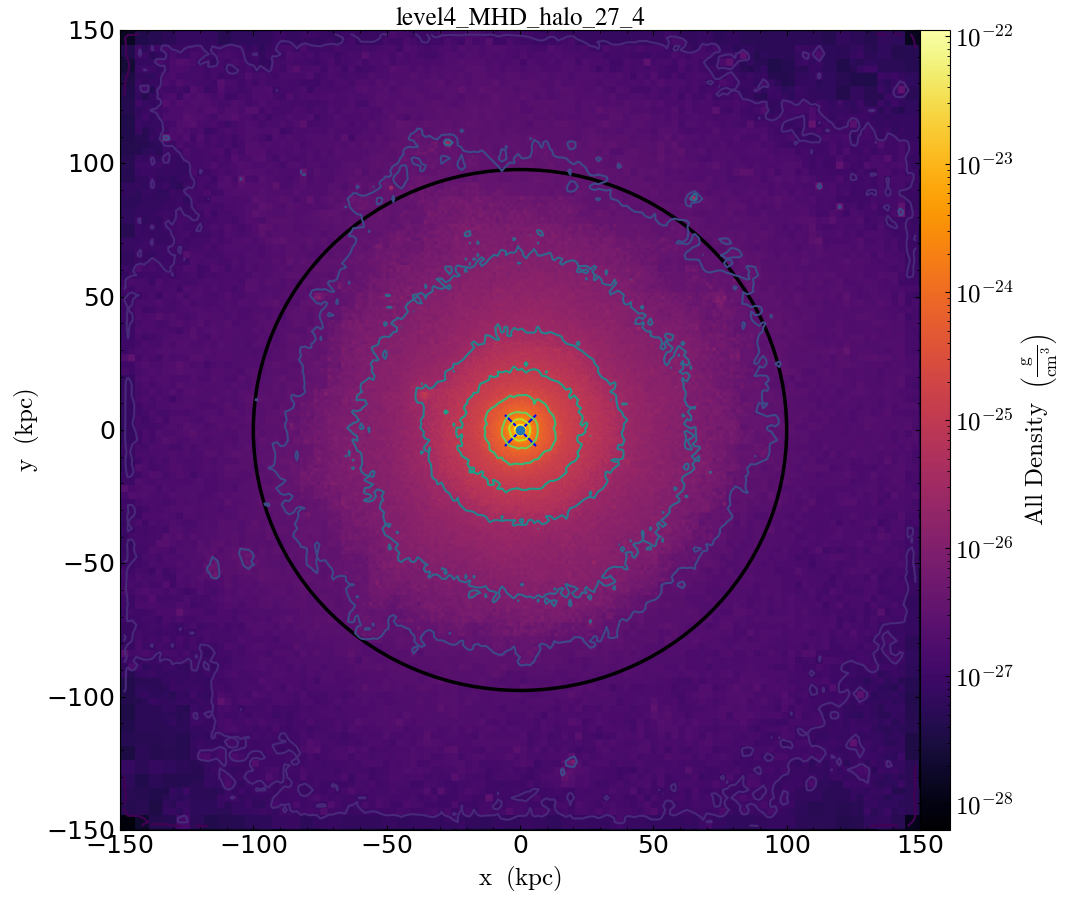
\includegraphics[width=0.38\columnwidth]{../Document/pics/MHD_Vs_DM/level4_MHD_halo_27_outter.png}}
 % \caption{DM density for inner (left) and outer (right) parts of the halo 27. We present both versions: DM (up) \& MHD (down). The horizontal and vertical axes are aligned to the major and medium semi-axes respectively. Here, it is evident that this halo is more spherical at bigger radii and more triaxial at the central parts. }
\normalsize
  \label{fig:slices}
\end{figure}
\centering
 \tiny Prada et al. 2018 (in process)

\end{frame}

\begin{frame}

\centering
MHD halos are more spherical than DM halos (scattering)
\begin{figure}[!ht]
  \centering
  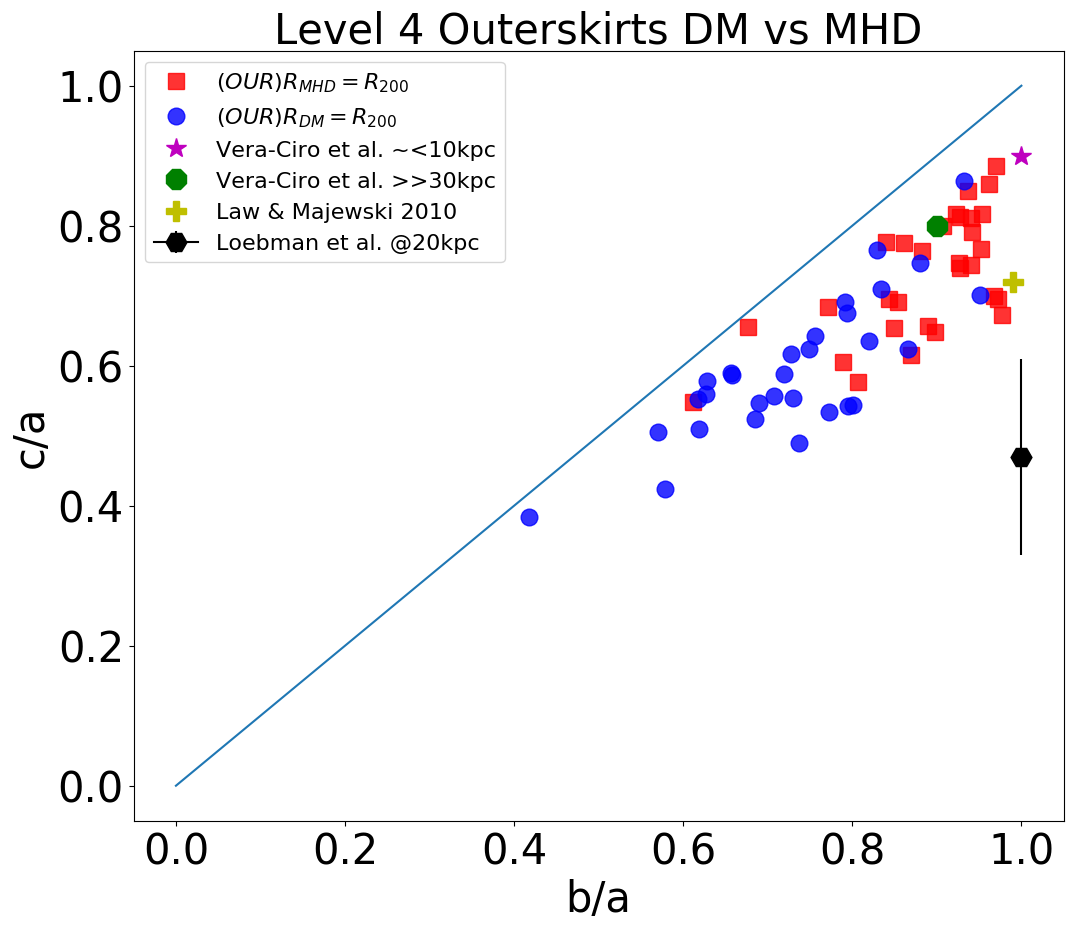
\includegraphics[width=0.6\columnwidth]{./pics/Triaxiality_Outter_lvl4.png}
  \caption{\tiny Prada et al. 2018 (in process)}
  \hfil
\end{figure}
\normalsize

\end{frame}

%---------------------------------------------------------------------------------------

%---------------------------------------------------------------------------------------
\subsection{Historical and radial correlations}
\begin{frame}
\centering
\LARGE
\textbf{Historical and radial correlations}
\normalsize
\end{frame}

\begin{frame}
\centering
Halos evolve towards more oblate shapes.
\begin{figure}[!ht]
  \centering
 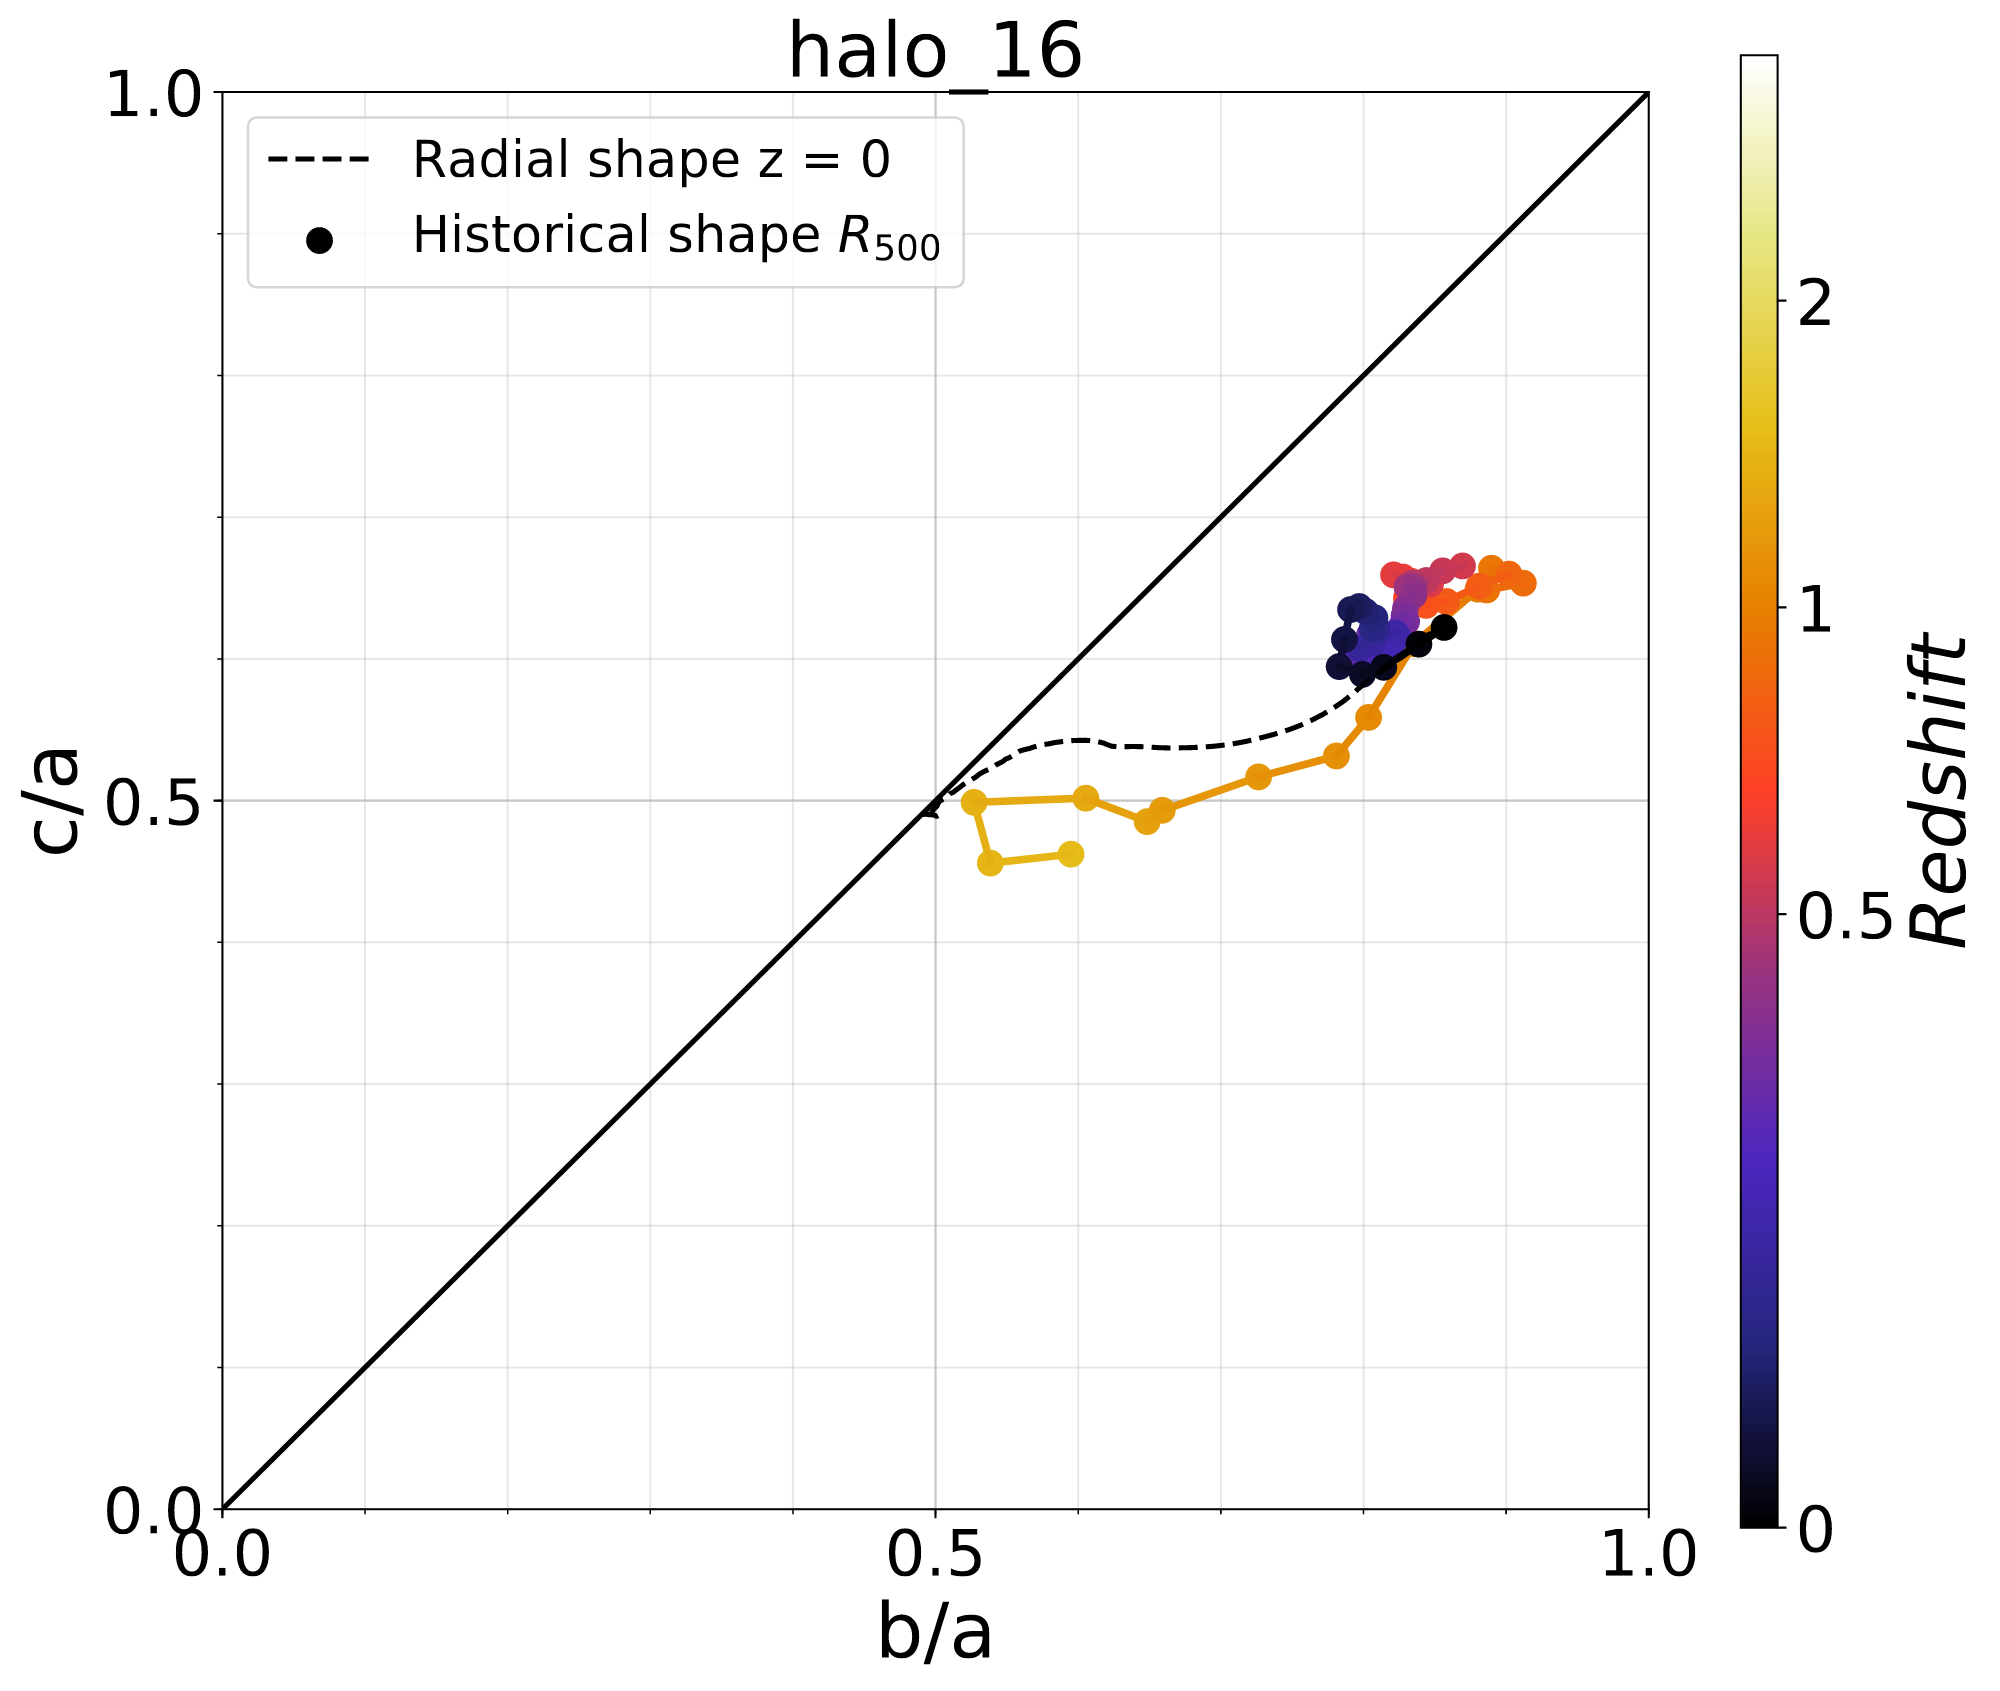
\includegraphics[width=0.6\columnwidth]{../Document/pics/Redshift/halo_16_level3_DM_Z_Triax.png}
 \caption{Halo 16 DM \tiny Prada et al. 2018 (in process)}
  
  %\caption{Historic shape (color dots) Vs actual radial shape (solid black line) on the Triaxiality plane. Each colored dot represents a calculated shape at R Mean 200, for each redshift. It is clear that halos with memory (halo 16), unlike disrupted halos (halo 21), have correlation between their historical and radial profiles.}
  \label{fig:RedshiftDM}
\end{figure}

\end{frame}


\begin{frame}
\centering
Reason: systematic tendence towards oblate/spherical shapes.
\begin{figure}[!ht]
  \centering
  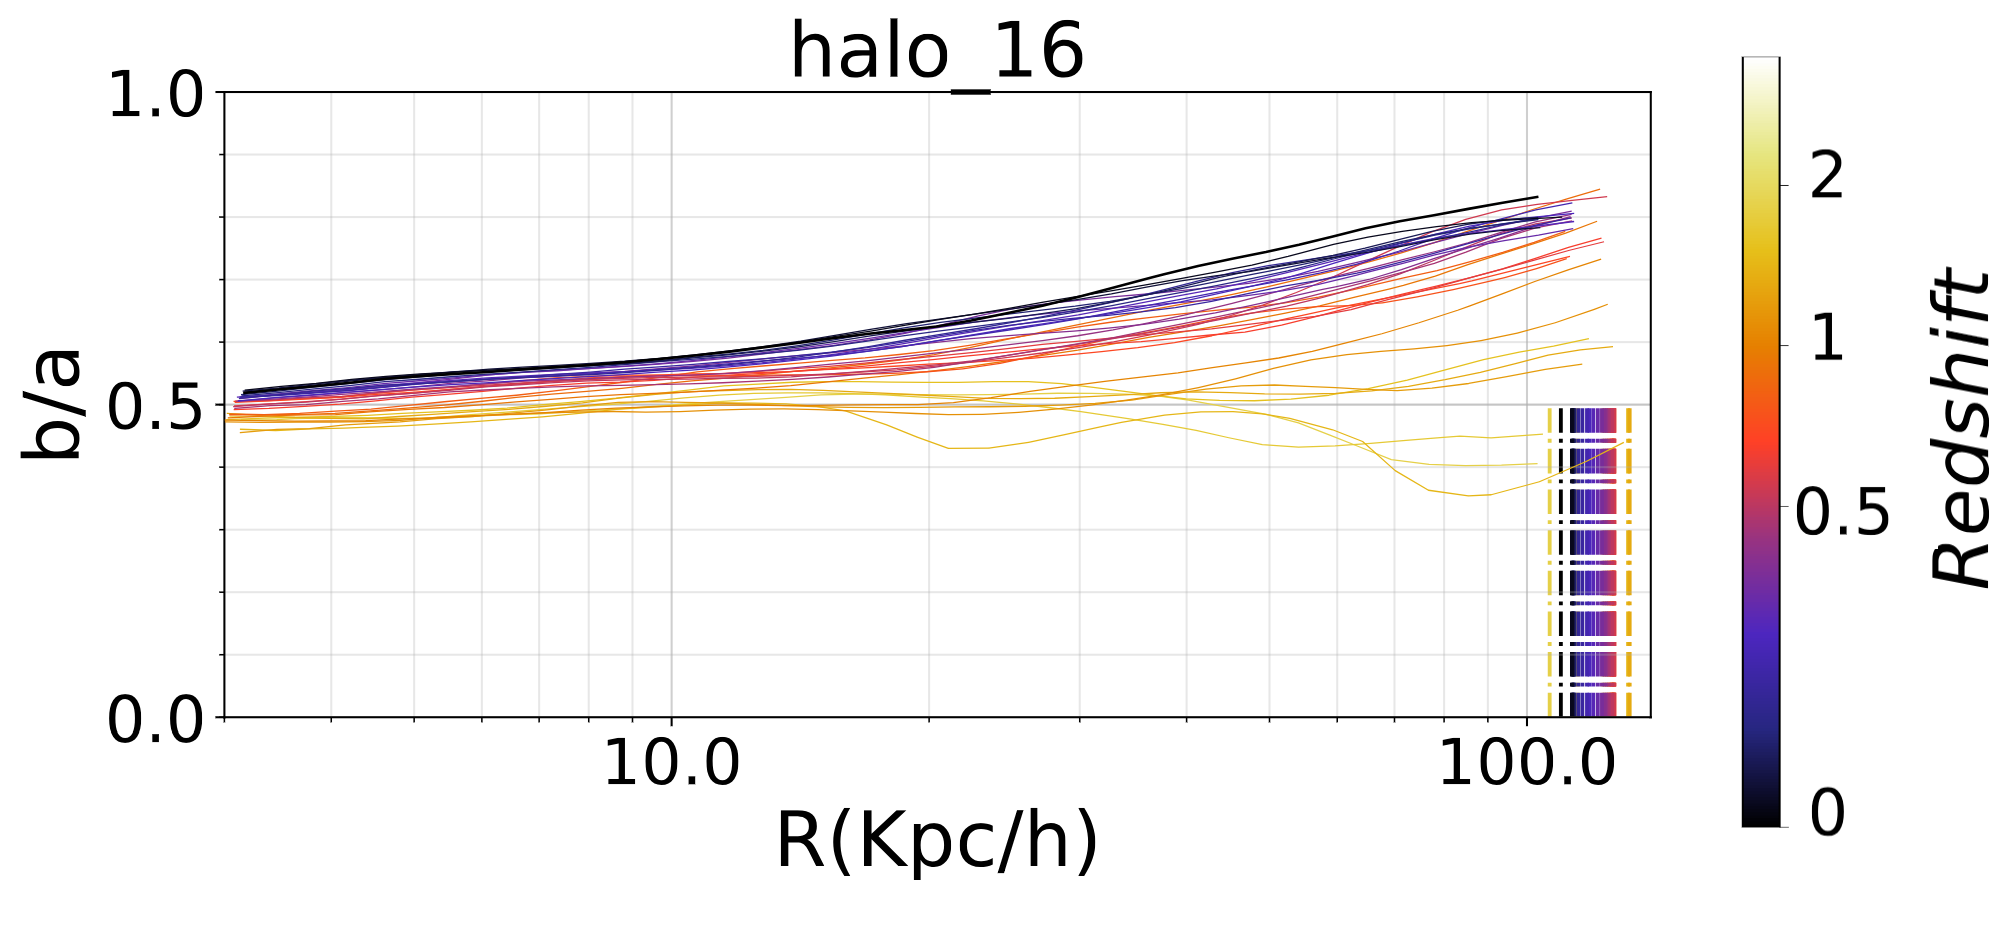
\includegraphics[width=1\columnwidth]{./pics/halo_16_level3_DM_Z.png}
  \caption{Halo 16 DM \tiny Prada et al. 2018 (in process)}
  \hfill

\end{figure}
\end{frame}

\begin{frame}
\centering
Example of shape \textit{memory} loss.
\begin{figure}[!ht]
  \centering
 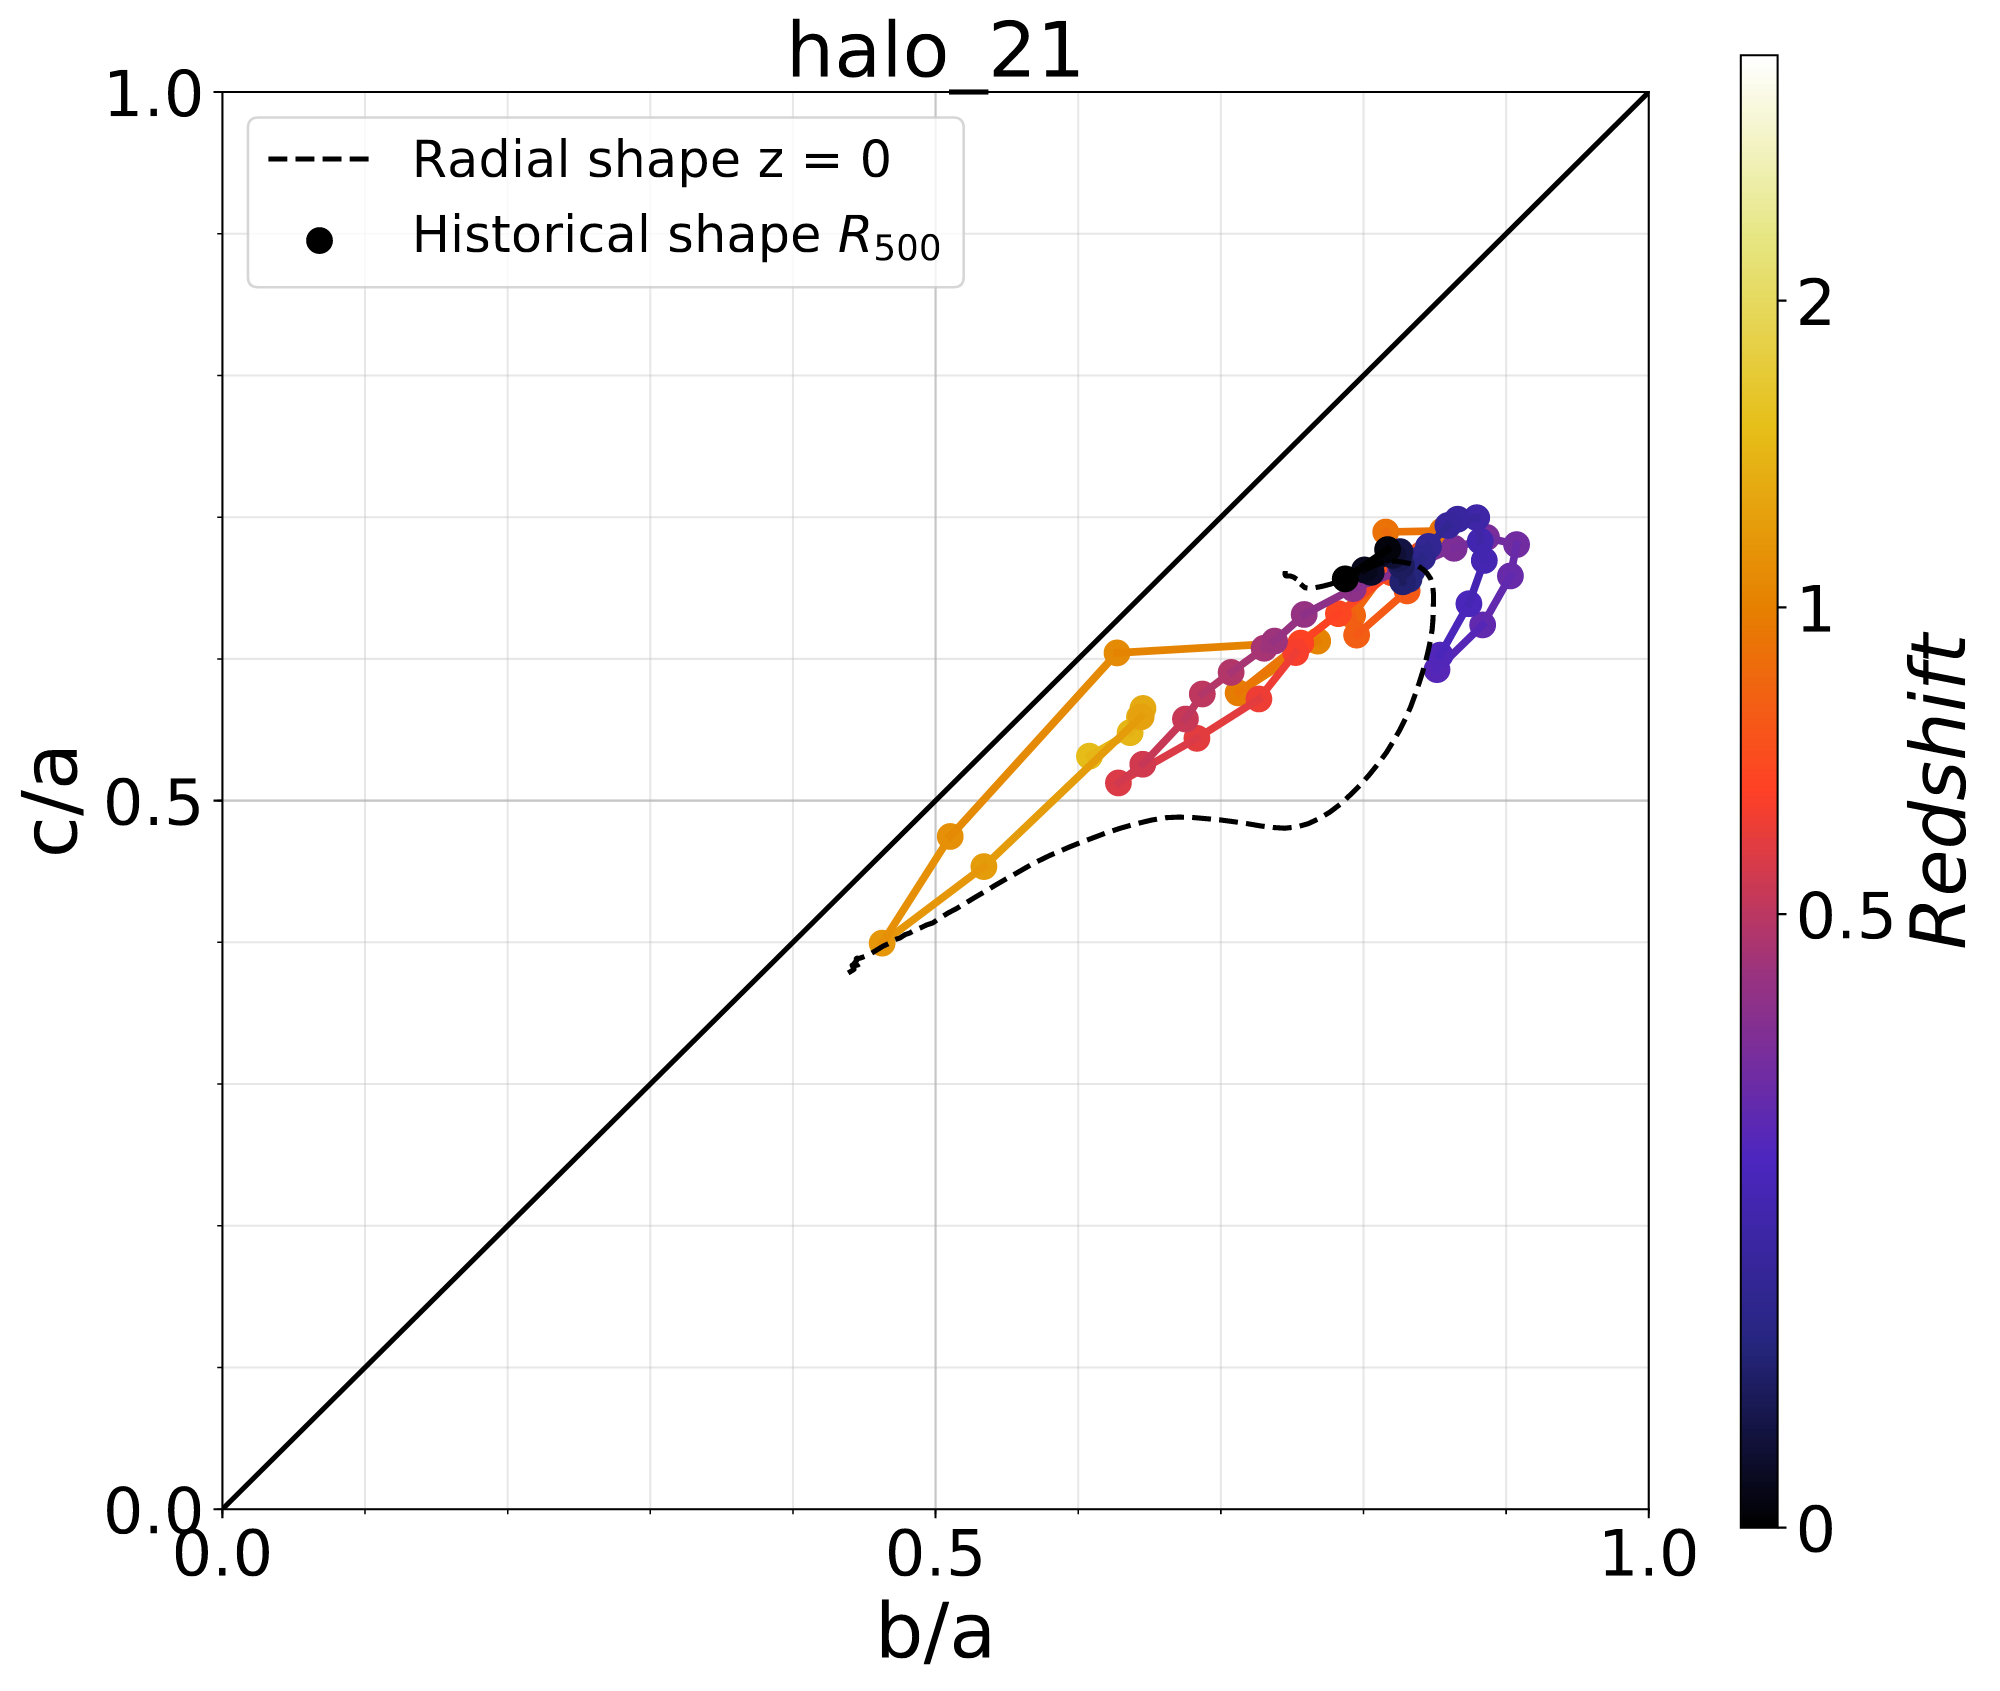
\includegraphics[width=0.6\columnwidth]{../Document/pics/Redshift/halo_21_level3_DM_Z_Triax.png}
 \caption{Halo 16 DM \tiny Prada et al. 2018 (in process)}
  

  \label{fig:RedshiftDM}
\end{figure}
\end{frame}


\begin{frame}
Major event? \textbf{Virial radius change}
\begin{figure}[!ht]
  \centering
  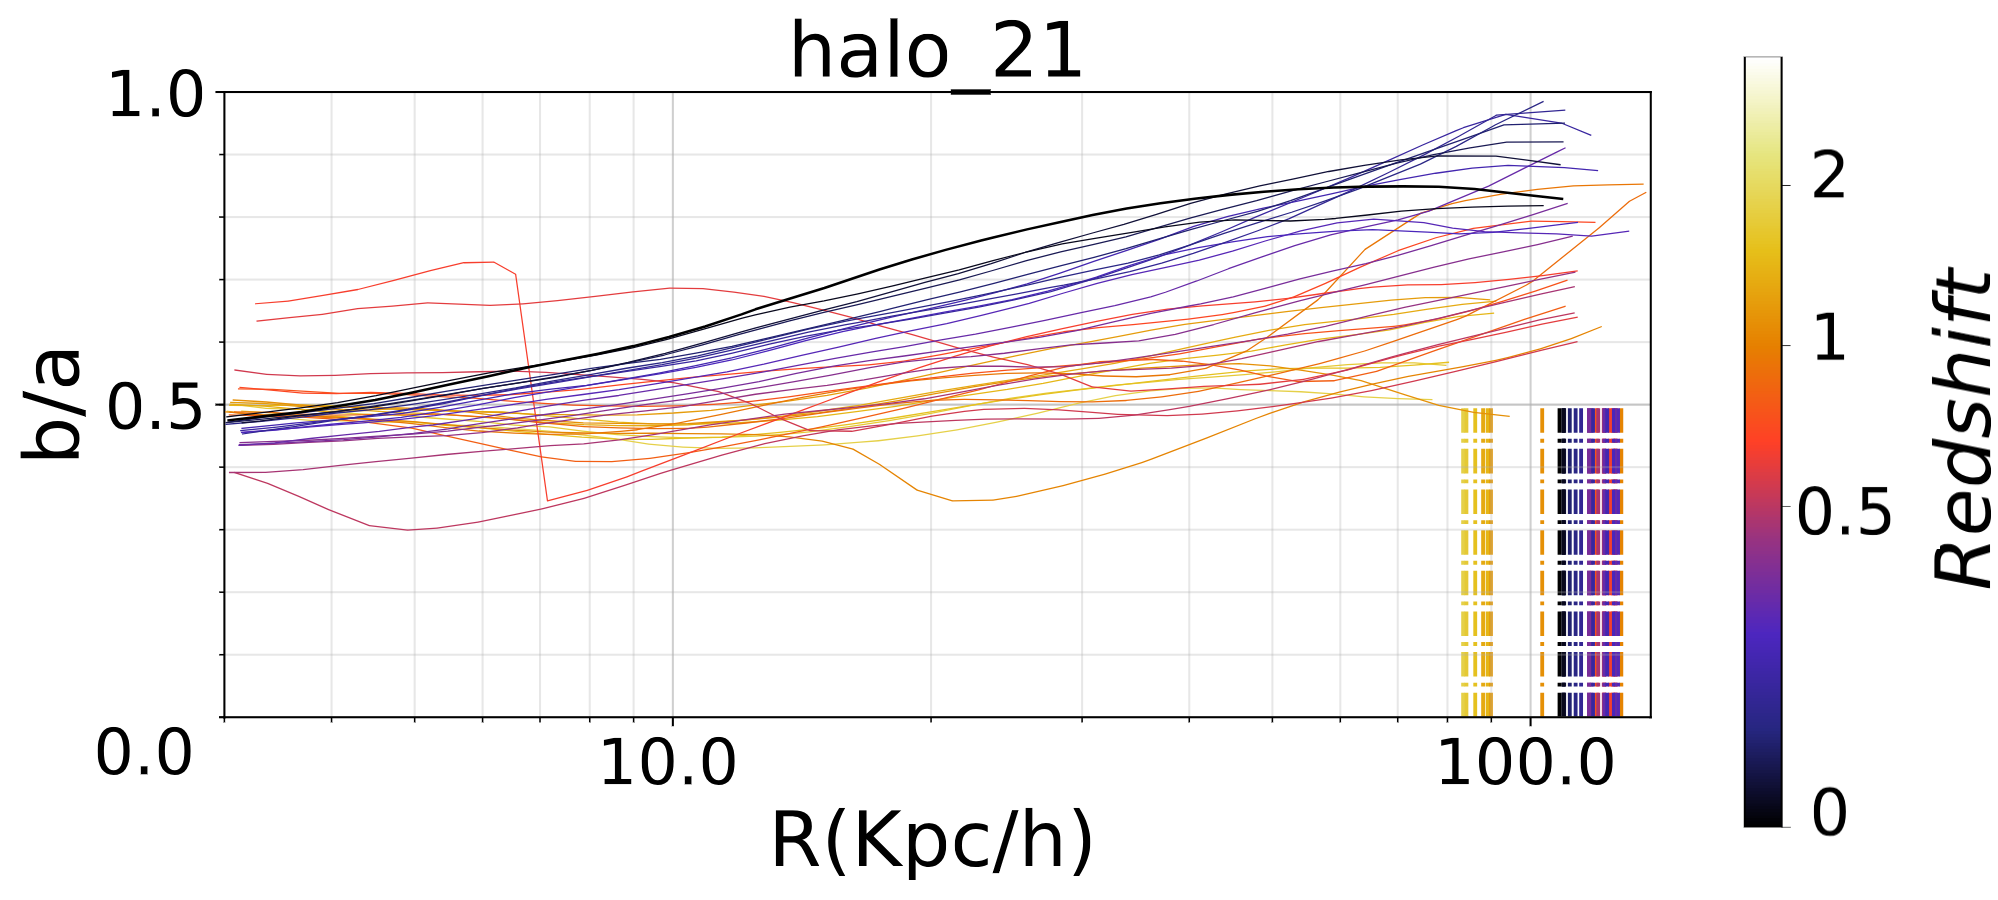
\includegraphics[width=1\columnwidth]{./pics/halo_21_level3_DM_Z.png}
  \caption{\tiny Prada et al. 2018 (in process)}
\end{figure}

\end{frame}

\begin{frame}[plain]

\begin{figure}[!ht]
  \centering
  \subfloat[\tiny halo 21 DM z=0]{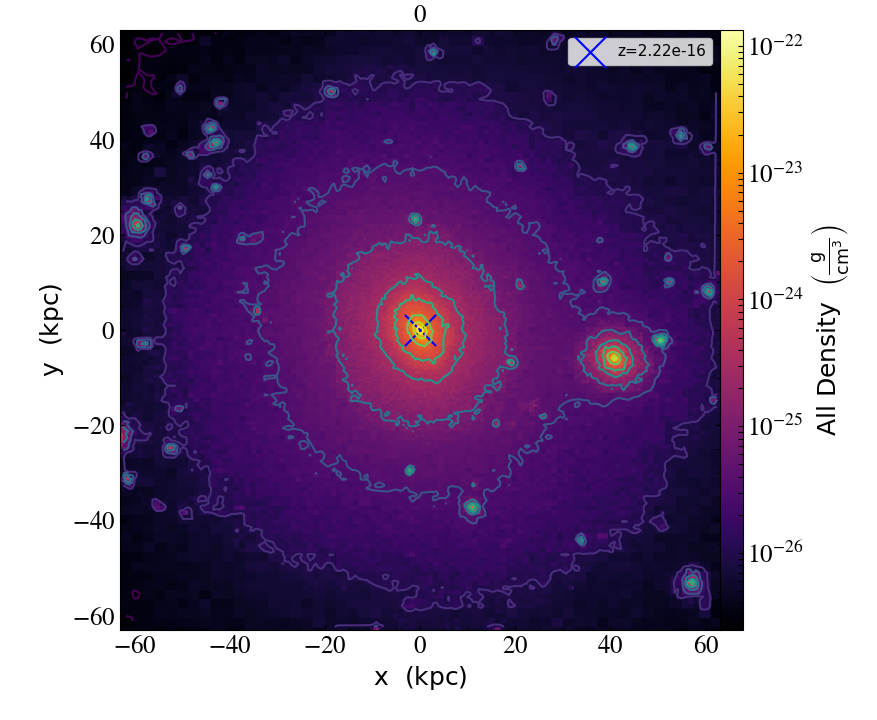
\includegraphics[width=0.38\columnwidth]{./pics/0.png}}
  \hfill
   \subfloat[\tiny halo 21 DM z=0.13]{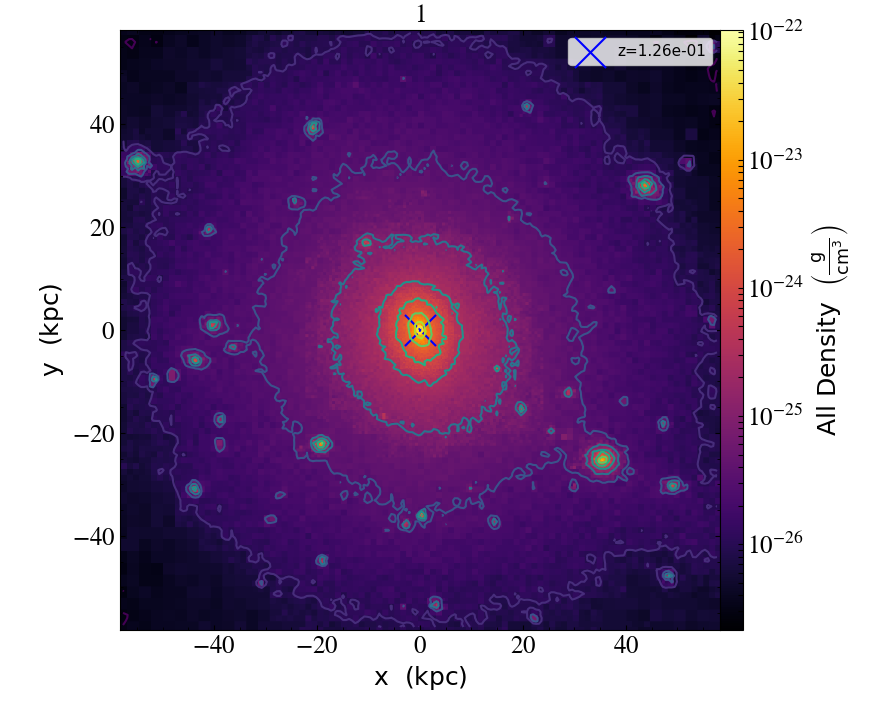
\includegraphics[width=0.38\columnwidth]{./pics/1.png}}
  \hfill
  \subfloat[\tiny halo 21 DM z=0.27]{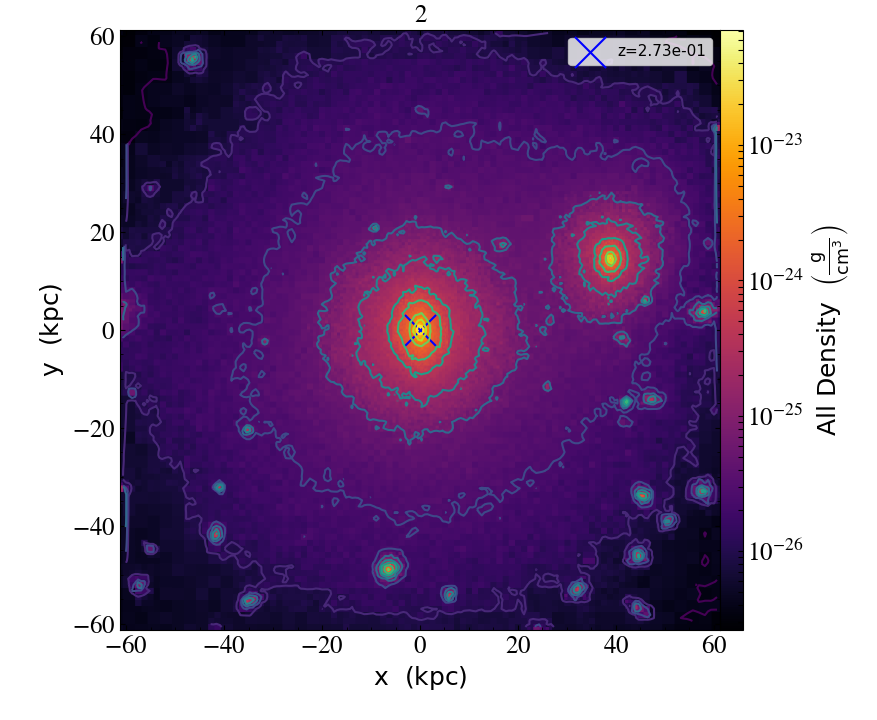
\includegraphics[width=0.38\columnwidth]{./pics/2.png}}
  \hfill
  \subfloat[\tiny halo 21 DM z=0.46]{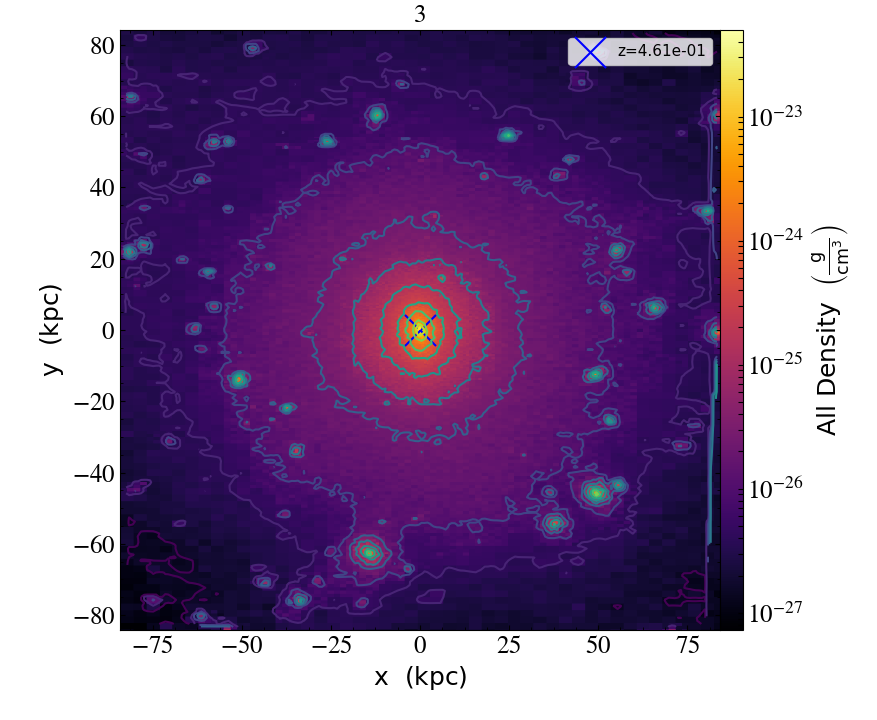
\includegraphics[width=0.38\columnwidth]{./pics/3.png}}
 % \caption{DM density for inner (left) and outer (right) parts of the halo 27. We present both versions: DM (up) \& MHD (down). The horizontal and vertical axes are aligned to the major and medium semi-axes respectively. Here, it is evident that this halo is more spherical at bigger radii and more triaxial at the central parts. }
\normalsize

\end{figure}
\centering \tiny Prada et al. 2018 (in process)


\end{frame}


%---------------------------------------------------------------------------------------
\section{Conclusions}
\begin{frame}
\centering
\LARGE
\textbf{Conclusions}
\normalsize
\end{frame}

\begin{frame}

\begin{itemize}

\item DM halos are more oblate/spherical at larger radii.\\~\\

\item There is a correlation between historical and radial shapes which is caused by the generalized tendency of halos to evolve towards spherical shapes.\\~\\

\item Presence of matter increases tendency towards sphericity (scattering) \\~\\

\item Our results are supported by a significant sample.

\end{itemize}

\end{frame}

\section{Future work}
\begin{frame}
\centering
\LARGE
\textbf{Future work}
\normalsize
\end{frame}

\begin{frame}

\begin{itemize}

\item Paper (In process)\\~\\

\item Study the effect of environmental structures on halo shape and orientation.\\~\\

\item Study the response of DM halos to the presence of matter (Adiabatic contraction).\\~\\


\end{itemize}

\end{frame}

%---------------------------------------------------------------------------------------

%---------------------------------------------------------------------------------------


%---------------------------------------------------------------------------------------

%---------------------------------------------------------------------------------------


%---------------------------------------------------------------------------------------

%---------------------------------------------------------------------------------------



\section{References}
\begin{frame}[t, allowframebreaks]
\frametitle{Referencias}
\tiny
\bibliographystyle{unsrt}
\bibliography{Bibliography}
\end{frame}
\end{document}
